%narms.tex, an example driver file for Balkema documents.

%use the following for A4 paper:
\documentclass[12pt,a4paper,twocolumn,fleqn]{narms}


% packages needed
%\usepackage{subfigure}
\usepackage{epsfig}
\usepackage{timesmt}
\mathindent=0pt%

\usepackage{chicaco}

% custom packages
\usepackage{amsmath}
\usepackage[noabbrev]{cleveref}
\usepackage{dsfont}
\setlength{\mathindent}{0cm}
%\usepackage{subfig}
\usepackage{graphicx}
\usepackage{subcaption}
\usepackage{siunitx}
\usepackage[font=small,justification=justified,singlelinecheck=false]{caption}


% setting math equation indent from left 0pts

\mathindent=0pt%

% use this for chicaco style reference
% Author references
% IMPORTANT: Author wants to format references in chicaco style Author must use BiBTex
% IMPORTANT: Author wants to format numbered references remove chicaco style file and \bibliographystyle{chicaco}

\usepackage{chicaco}

%  \cite{key}
%    which produces citations with full author list and year.
%    eg. (Brown 1978; Jarke, Turner, Stohl, et al. 1985)

%  \citeNP{key}
%    which produces citations with full author list and year, but without
%    enclosing parentheses:
%    eg. Brown 1978; Jarke, Turner & Stohl 1985

%  \citeA{key}
%    which produces citations with only the full author list.
%    eg. (Brown; Jarke, Turner & Stohl)

%  \citeANP{key}
%    which produces citations with only the full author list, without
%    parentheses eg. Brown; Jarke, Turner & Stohl

%  \citeN{key}
%    which produces citations with the full author list and year, but
%    can be used as nouns in a sentence; no parentheses appear around
%    the author names, but only around the year.
%      eg. Shneiderman (1978) states that......
%    \citeN should only be used for a single citation.

%  \shortcite{key}
%    which produces citations with abbreviated author list and year.

%  \shortciteNP{key}
%    which produces citations with abbreviated author list and year.

%  \shortciteA{key}
%    which produces only the abbreviated author list.

%  \shortciteANP{key}
%    which produces only the abbreviated author list.

%  \shortciteN{key}
%    which produces the abbreviated author list and year, with only the
%    year in parentheses. Use with only one citation.

%  \citeyear{key}
%    which produces the year information only, within parentheses.

%  \citeyearNP{key}
%    which produces the year information only.


%%%%%%%%%%%%%%%%%%%%%%%%%%%%%%%%%%%%%%%%%%%%%%%%%%%%%%%%%%%%%%%%%%%
%%%  All this stuff is from modifying the article.cls for Balkema
%%%  specifications.

%\title{...}
%\author{...}
%use \aff for author affiliations
% use \authornext for from second author
% empty line space between multiple authors
%\abstract{...}
%\maketitle{}

%%%%%%% Style for TABLES
% insert tabular command inside \tabletext{} this will produce tables in 10pts


\begin{document}
\title{Effect of initial volume fraction on the collapse of granular columns in fluid}
\author{{K. Kumar} \\
{\aff{Computational Geomechanics Research Group, Department of Engineering, University of Cambridge, UK}} \\
\\
{\authornext{J-Y. Delenne}}\\
{\aff{IATE, UMR 1208 INRA-CIRAD-Montpellier Supagro-UM2, University of Montpellier 2, France.}} \\
\\
{\authornext{K. Soga}}\\
{\aff{Department of Civil and Environmental Engineering, University of California, Berkeley, USA.}}}

\date{}% No date.

\abstract{This paper investigates the effect of initial volume fraction on the runout characteristics of granular column collapse in a fluid. Two-dimensional sub-grain scale numerical simulations are performed to understand the flow dynamics of granular collapse in a fluid. The Discrete Element (DEM) technique is coupled with the Lattice Boltzmann Method (LBM), for fluid-grain interactions, to understand the evolution of submerged granular flows. The fluid phase is simulated using Multiple-Relaxation-Time LBM (LBM-MRT) for numerical stability. In order to simulate interconnected pore space in 2D, a reduction in the radius of the grains (hydrodynamic radius) is assumed during LBM computations. A parametric analysis is performed to assess the influence of the granular characteristics (initial packing) on the evolution of flow and run-out distances. The volume of the initial packing is changed to simulate different stress conditions while maintaining the same aspect ratio. The influence of the stress condition on the run-out behaviour is studied for different permeabilities. The granular flow dynamics is investigated by analysing the effect of hydroplaning, water entrainment and viscous drag on the granular mass. The mechanism of energy dissipation, the shape of the flow front, water entrainment and evolution of packing density is used to explain the difference in the flow characteristics of loose and dense granular column collapse in a fluid.}

\maketitle

\section{INTRODUCTION}


The flow of dense granular material is a common phenomenon in engineering predictions, such as avalanches, landslides, and debris-flow modelling. Despite the huge amount of research that has gone into describing the behaviour of granular flows, a constitutive equation that describes the overall behaviour of a flowing granular material is still lacking. The initiation and propagation of submarine granular flows depend mainly on the slope, density, and quantity of the material destabilised. Although certain macroscopic models are able to capture the simple mechanical behaviours, the complex physical mechanisms that occur at the grain scale, such as thydrodynamic instabilities, the formation of clusters, collapse, and transport, have largely been ignored~\shortcite{Topin2011}. The momentum transfer between the discrete and the continuous phases significantly affects the dynamics of the flow~\shortcite{Peker2007}. Grain-scale description of the granular material enriches the macro-scale variables,  which poorly account for the local rheology of the materials.  In order to describe the mechanism of saturated and/or immersed granular flows, it is important to consider both the dynamics of the solid phase and the role of the ambient fluid~\shortcite{Denlinger2001}. In particular, when the solid phase reaches a high volume fraction, it is important to consider the strong heterogeneity arising from the contact forces between the grains, the drag interactions which counteract the movement of the grains, and the hydrodynamic forces that reduce the weight of the solids inducing a transition from dense compacted to a dense suspended flow~\shortcite{Meruane2010}. The case of the collapse in presence of an interstitial fluid has been less studied. In this paper, we study the submarine granular flows in the inclined configuration. We study the effect of permeability, density and slope angle on the run-out evolution.
\section{LBM FORMULATION}

The Lattice Boltzmann Method is a `micro-particle' based numerical time-stepping procedure for the solution of incompressible fluid flows. Consider a 2D incompressible fluid flow with density $\rho$ and kinematic viscosity \textit{v}, in a rectangular domain \textit{\textbf{D}}. The fluid domain is divided into a rectangular grid or lattice, with the same spacing \textit{`h'} in both the \textit{x-} and the \textit{y-}directions, as shown in~\cref{fig:D2Q9}. The present study focuses on two-dimensional problems, hence the \textit{D2Q9} momentum discretisation is adopted (see \shortciteN{He1997} for naming convention).

\begin{figure}[htpb]
\centering
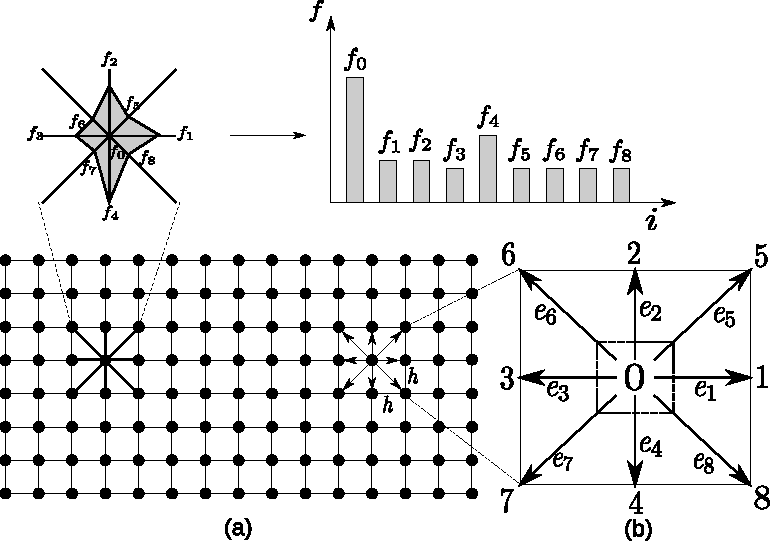
\includegraphics[width=0.45\textwidth]{figs/D2Q9.pdf}
\caption[The Lattice Boltzmann discretisation and D2Q9 scheme]{The Lattice Boltzmann discretisation and D2Q9 scheme: (a) a standard LB lattice and histogram views of the discrete single particle distribution function/direction-specific densities $f_i$; (b) D2Q9 model}
\label{fig:D2Q9}
\end{figure}

The lattice Boltzmann Bhatnagar-Gross-Krook (LGBK) method is capable of simulating various hydrodynamics~\shortcite{Succi2001} and offers intrinsic parallelism. Although LBM is successful in modelling complex fluid systems, such as multiphase flows and suspensions in fluid, the LBM may lead to numerical instability when the dimensionless relaxation time $\tau$ is close to 0.5. The Multi-Relaxation Time Lattice Boltzmann Method (LBM-MRT) overcomes the deficiencies of linearlised single relaxation LBM-BGK, such as fixed Prandtl number (Pr=$\nu/\kappa$), where the thermal conductivity `$\kappa$' is unity~\shortcite{Liu2003a}. The LB-MRT model offers better numerical stability and has more degrees of freedom. In the formulation of the linear Boltzmann equation with multiple relaxation time approximation, the lattice Boltzmann equation is written as:

\begin{align}
&f_{\alpha}(\mathbf{x}+\mathbf{e}_i\Delta_t, t+ \Delta_t)-f_{\alpha}(\mathbf{x},t) \nonumber \\
&\mbox{\qquad\qquad} = -\mathbf{S}_{\alpha i}(f_i(\mathbf{x},t)-f_i^{eq}(\mathbf{x},t)
\end{align}

\noindent where \textbf{S} is collision matrix. The nine eigen values of \textbf{S} are all between 0 and 2 so as to maintain linear stability and the separation of scales, which means that the relaxation times of non-conserved quantities are much faster than the hydrodynamic time scales. The LGBK model is the special case in which the nine relaxation times are all equal and the collision matrix $\mathbf{S}=\frac{1}{\tau}\mathbf{I}$, where \textbf{I} is the identity matrix. The evolutionary progress involves two steps, advection and flux. The advection can be mapped to the momentum space by multiplying through by a transformation matrix \textbf{M} and the flux is still finished in the velocity space. The evolutionary equation of the multi-relaxation time lattice Boltzmann equation is written as:

\begin{align}
&\mathbf{f}(\mathbf{x}+\mathbf{e}_i\Delta_t, t+ \Delta_t)-\mathbf{f}(\mathbf{x},t) \nonumber \\
&\mbox{\qquad\qquad} = -M^{-1}\hat{\mathbf{S}} (\hat{\mathbf{f}}(\mathbf{x},t)-\hat{\mathbf{f}}^{eq}(\mathbf{x},t))
\end{align}

\noindent where \textbf{M} is the transformation matrix mapping a vector \textbf{f} in the discrete velocity space $\mathds{V}=\mathds{R}^b$ to a vector $\hat{\mathbf{f}}$ in the moment space $\mathds{V}=\mathds{R}^b$.

\begin{align}
&\hat{\mathbf{f}} = \mathbf{M}\mathbf{f}\\
&\mathbf{f}(\mathbf{x},t) = \left[f_0(\mathbf{x},t),f_1(\mathbf{x},t),\dots f_8(\mathbf{x},t)\right]^T
\end{align}

The collision matrix $\hat{\mathbf{S}} = MSM^{-1}$ in moment space is a diagonal matrix: $\hat{\mathbf{S}} =\mbox{diag} \left[ s_1, s_2, s_3,\dots s_9  \right]$. The transformation matrix \textbf{M} can be constructed via Gram-Schmidt orthgonalisation procedure. Through the Chapman-Enskog expansion~\shortcite{Du2006}, the incompressible Navier-Stokes equation can be recovered and the viscosity is given as:
\begin{align}
\nu=c_s^2\Delta t(\tau-0.5)
\end{align}
%**************************************************************************

\subsection{Turbulence in Lattice Boltzmann Method}
Modelling fluids with low viscosity like water remains a challenge, necessitating very small values of \textit{h}, and/or $\tau$ very close to 0.5~\shortcite{He1997}. Turbulent flows are characterised by the occurrence of eddies with multiple scales in space, time and energy. In this study, the Large Eddy Simulation (LES) is adopted to solve for turbulent flow problems. The separation of scales is achieved by filtering of the Navier-Stokes equations, from which the resolved scales are directly obtained and unresolved scales are modelled by a one-parameter Smagorinski sub-grid methodology, which assumes that the Reynold's stress tensor is dependent only on the local strain rate~\shortcite{Smagorinsky1963}. The turbulent viscosity $\nu$ is related to the strain rate $S_{ij}$ and a filtered length scale `h' as follows:
\begin{align}
&\mathit{v}_{\mathit{t}}  =  (\mathit{S}_{c}\mathit{h})^{2}\overline{S}; \\
&\overline{S}  = \sqrt{\sum\limits_{\mathit{i,j}}{\tilde{S}_{\mathit{i,j}}\tilde{S}_{\mathit{i,j}}}}
\end{align}
where $\mathit{S}_{c}$ is the Smagorinski constant found to be close to 0.03~\shortcite{yu2005}.

The effect of the unresolved scale motion is taken into account by introducing an effective collision relaxation time scale $\tau_{t}$, so that the total relaxation time $\tau_{*}$ is written as:
\begin{align}
\tau_{*}=\tau + \tau_{t}
\end{align}
where $\tau$ and $\tau_{t}$ are respectively the standard relaxation times corresponding to the true fluid viscosity \textit{v} and the turbulence viscosity $\mathit{v}_{\mathit{t}}$, defined by a sub-grid turbulence model. The new viscosity $\mathit{v}_{*}$ corresponding to $\tau_{*}$ is defined as:
\begin{align}
& \mathit{v}_{*}=\mathit{v}+\mathit{v}_{\mathit{t}}=\frac{1}{3}(\tau+\tau_{t}-\frac{1}{2})\mathit{C}^{2} \Delta \mathit{t}  \\
& \mathit{v}_{\mathit{t}}=\frac{1}{3}\tau_{\mathit{t}}\mathit{C}^{2} \Delta \textit{t}
\end{align}
The Smagorinski model is easy to implement and the Lattice Boltzmann formulation remains unchanged, except for the use of a new turbulence-related viscosity $\tau_{*}$. The component $s_1$ of the collision matrix becomes $s_1 = \frac{1}{\tau+\tau_t}$.
%************************************************************************* %
\section{COUPLED LB - DEM FOR FLUID-PARTICLE INTERACTIONS}
The Lattice Boltzmann approach has the advantage of accommodating large particle sizes and the interaction between the fluid and the moving particles can be modelled through relatively simple fluid - particle interface treatments. Further, employing the Discrete Element Method (DE) to account for the particle/particle interaction naturally leads to a combined LB - DEM solution procedure. The Eulerian nature of the Lattice Boltzmann formulation, together with the common explicit time step scheme of both the Lattice Boltzmann and the Discrete Element makes this coupling strategy an efficient numerical procedure for the simulation of particle-fluid systems~\shortcite{Cook2004}. In order to capture the actual physical behaviour of the fluid-particle system, the boundary condition between the fluid and the particle is modelled as a non-slip boundary condition, i.e. the fluid near the particle should have similar velocity as the particle boundary. The solid particles inside the fluid are represented by lattice nodes. The discrete nature of lattice will result in stepwise representation of the surfaces. Very small lattice spacing is adopted to obtain smoother boundaries.

\section{UNDERWATER GRANULAR FLOWS}
In this study, a 2D poly-disperse system ($d_{max}/d_{min} = 1.8$) of circular discs in fluid was used to understand the behaviour of granular flows on inclined planes (see~\Cref{fig:setup}). The soil column was modelled using 1000 discs of density \SI{2650}{\kg\per\cubic\meter} and a contact friction angle of \SI{26}{\degree}. The collapse of the column was simulated inside a fluid with a density of \SI{1000}{\kg\per\cubic\meter}  and a kinematic viscosity of \SI{1e-6}{\square\meter\per\second}. The choice of a 2D geometry has the advantage of cheaper computational effort than a 3D case, making it feasible to simulate very large systems. A granular column of aspect ratio `a' of 0.8 was used. A hydrodynamic radius r = 0.9R was adopted during the LBM computations. Dry analyses were also performed to study the effect of hydrodynamic forces on the run-out distance.

\begin{figure}[htpb]
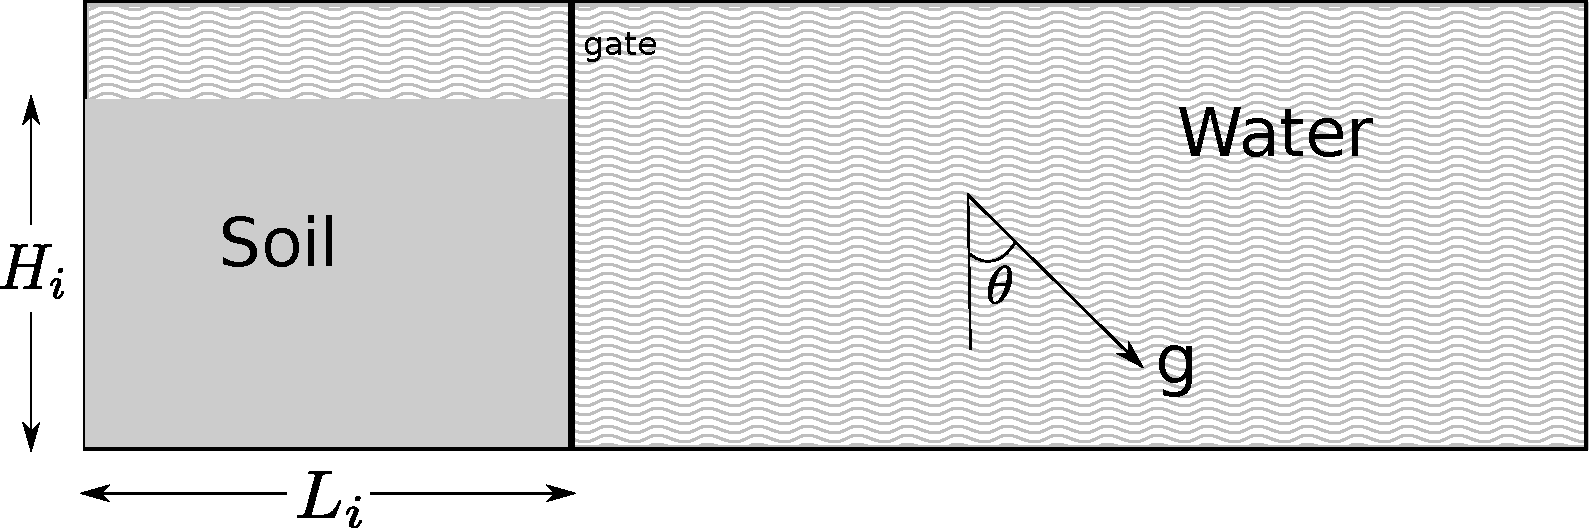
\includegraphics[width=0.97\columnwidth]{figs/geometry.pdf}
\caption{Underwater granular collapse set-up}
\label{fig:setup}
\end{figure}

\subsection{Effect of initial packing density}

\citeNP{Rondon2011} observed that the loose packings flow rapidly on a time
scale proportional to the initial height and results in longer run-out distance 
in comparison to the dense packing. Hydroplaning occurs above a critical 
Froude's number of 0.4. The Froude's number is inversely related to the 
thickness of the flow and its density. Hence, for the same thickness of flow, a 
loose granular column will experience more hydroplaning than a dense granular 
flow. This effect might result in longer run-out behaviour in fluid than the 
dry condition for the same initial aspect ratio. The initial packing density 
and the permeability of a 2D granular column, with an aspect ratio of 0.8, are 
varied to understand their influence on the run-out behaviour. The run-out 
behaviour of the dense case (83\% packing density), discussed in the previous 
section, is compared with a loose granular column (79\% packing fraction). The 
permeability is varied by changing the hydrodynamic radius from 0.7 \textit{R} 
to 0.95 
R. 

The normalised run-out evolution with time for a loose initial packing (79\% 
packing fraction) with different hydrodynamic radii 0.7 \textit{R}, 0.8 
\textit{R}, 0.9 and 0.95 R are presented in~\cref{fig:Runout_a08_loose}. The 
run-out evolution a column of grains in suspension is compared with the dry and 
submerged granular columns to understand the influence of hydrodynamic forces 
on the flow kinematics. Similar to the dense granular column, the run-out 
distance increases with increase in the hydrodynamic radius (i.e., decrease in 
permeability). At low permeabilities (\textit{r} = 0.9 and 0.95 \textit{R}), 
the run-out distance is longer than the dry condition. This shows that the 
lubrication effect in low permeability conditions overcomes the influence of 
the drag force and the development of large negative pore-pressure resulting in 
a longer run-out distance. Although the suspended granular masses experience 
higher drag forces and turbulent effects, the run-out evolves almost at the 
same rate in comparison with granular columns with high permeability. This 
shows the effect of permeability on the dissipation rate of negative 
pore-pressure developed during the initial stage of collapse.

\begin{figure}
\centering
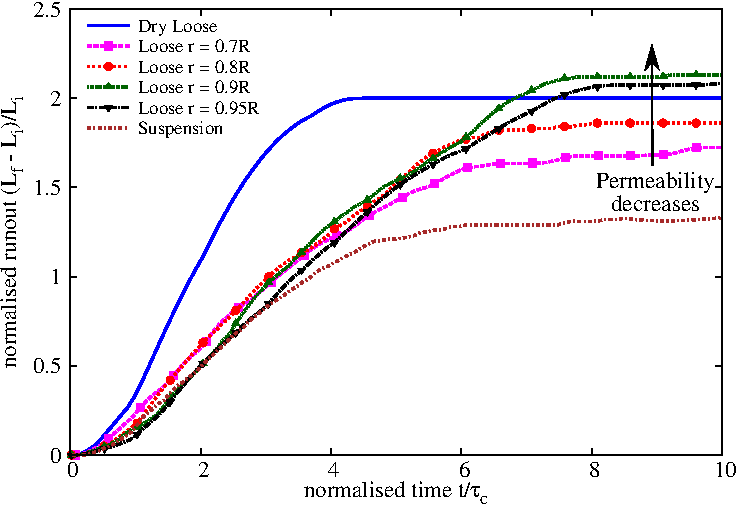
\includegraphics[width=0.9\linewidth]{figs/Runout_a08_loose.pdf}
\caption{Effect of permeability on the evolution of run-out for a column 
collapse in fluid (a = 0.8 \& loose packing).}
\label{fig:Runout_a08_loose}
\end{figure}

\Cref{fig:Loose_PWP_ini} shows the development of negative pore-pressure in low 
permeability (\textit{r} = 0.95 \textit{R}) and dissipation of negative 
pore-pressure in high permeability (\textit{r} = 0.7 \textit{R}) at the same 
time $ t = \tau_c$. This difference in the quantity and the rate of dissipation 
of negative pore-pressure results in a difference in the rate of flow 
evolution. A low permeability column requires a longer duration to 
evolve.~\Cref{fig:Loose_PWP_flow} shows the distribution of the excess 
pore-pressure along the bottom for low and high permeability conditions. As the 
flow progresses, the low permeability of the granular column causes 
hydroplaning to occur at the base of the column, which can be observed by high 
positive pore-pressure at the base of the flow front 
(\cref{fig:Loose_r095_PWP_flow,fig:Loose_r095_PWPress_flow}), resulting in a 
longer run-out distance.

\begin{figure}
\centering
\makebox[\linewidth][c]{
\begin{subfigure}[t]{0.975\linewidth}
	\centering
    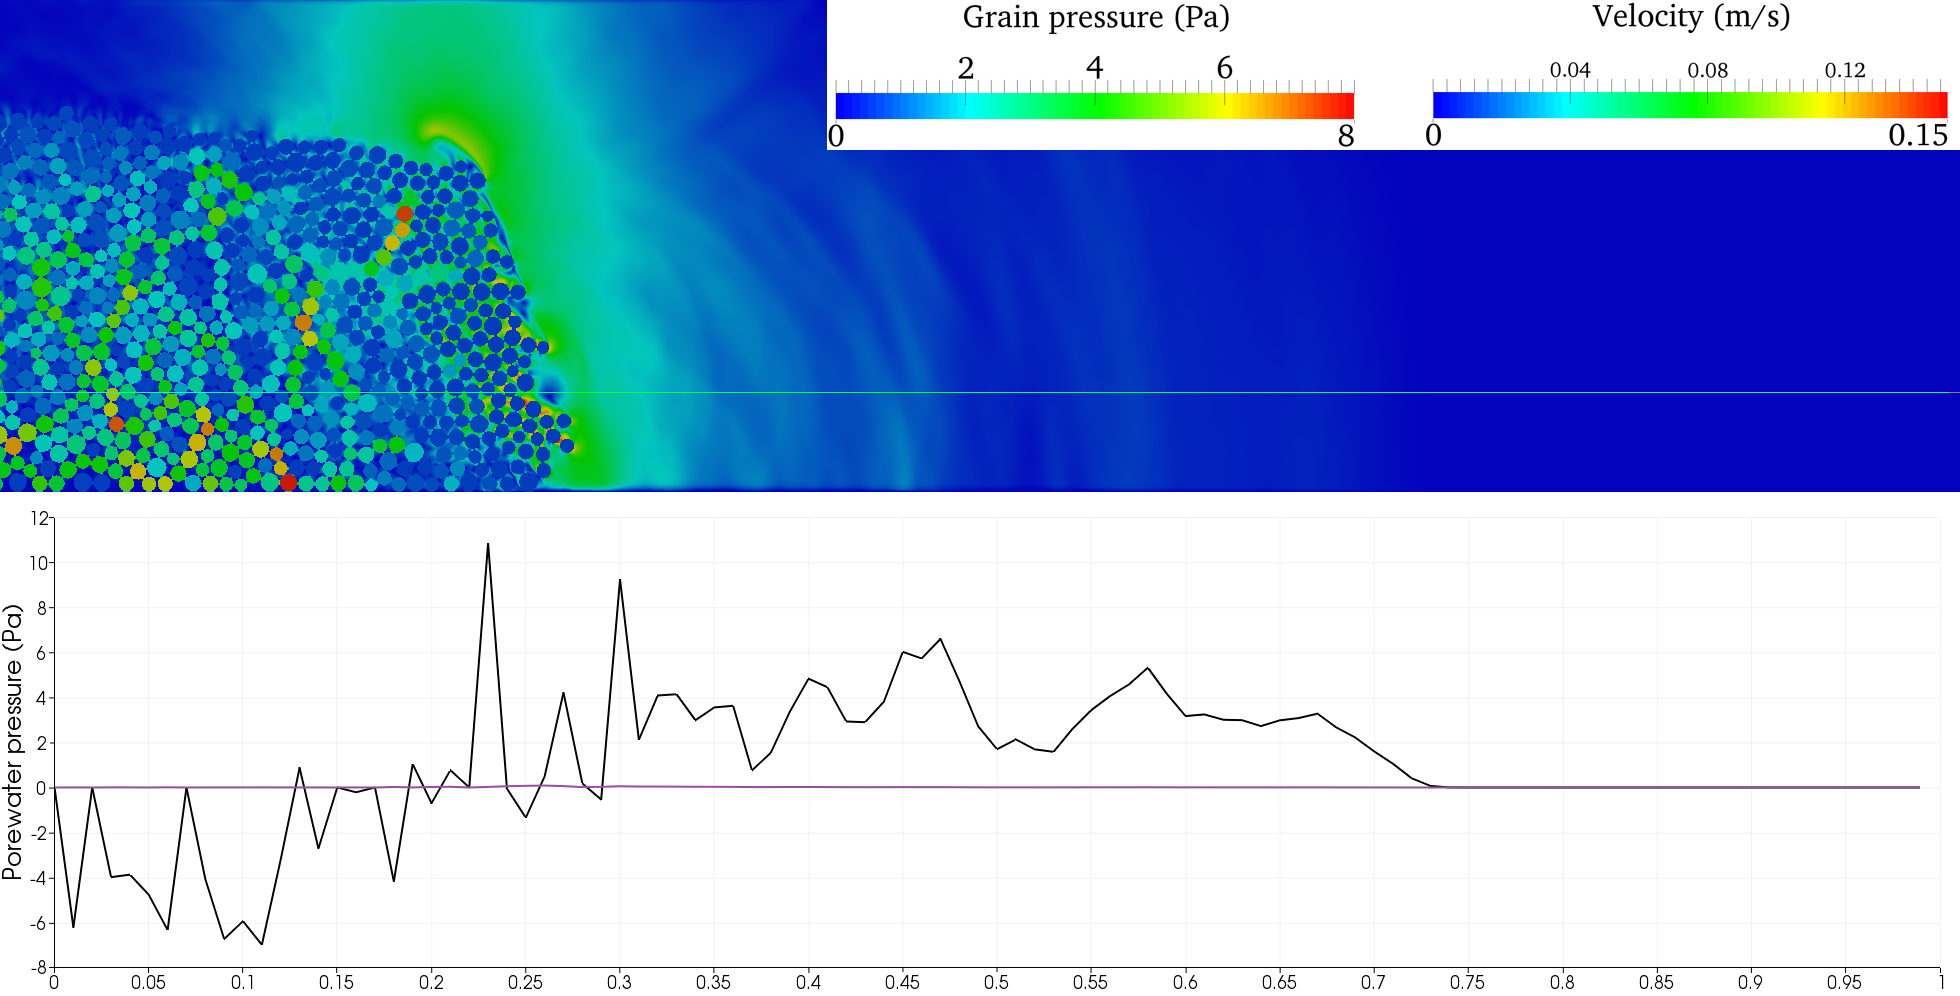
\includegraphics[width=\linewidth]{figs/a08/Loose_r07_PWP_ini}
    \caption{High permeability (\textit{r} = 0.7 \textit{R}) - Pressure at the 
        bottom of the granular flow.}
    \label{fig:Loose_r07_PWP_ini}
\end{subfigure}
}\\
\makebox[\linewidth][c]{
\begin{subfigure}[t]{0.975\linewidth}
	\centering
    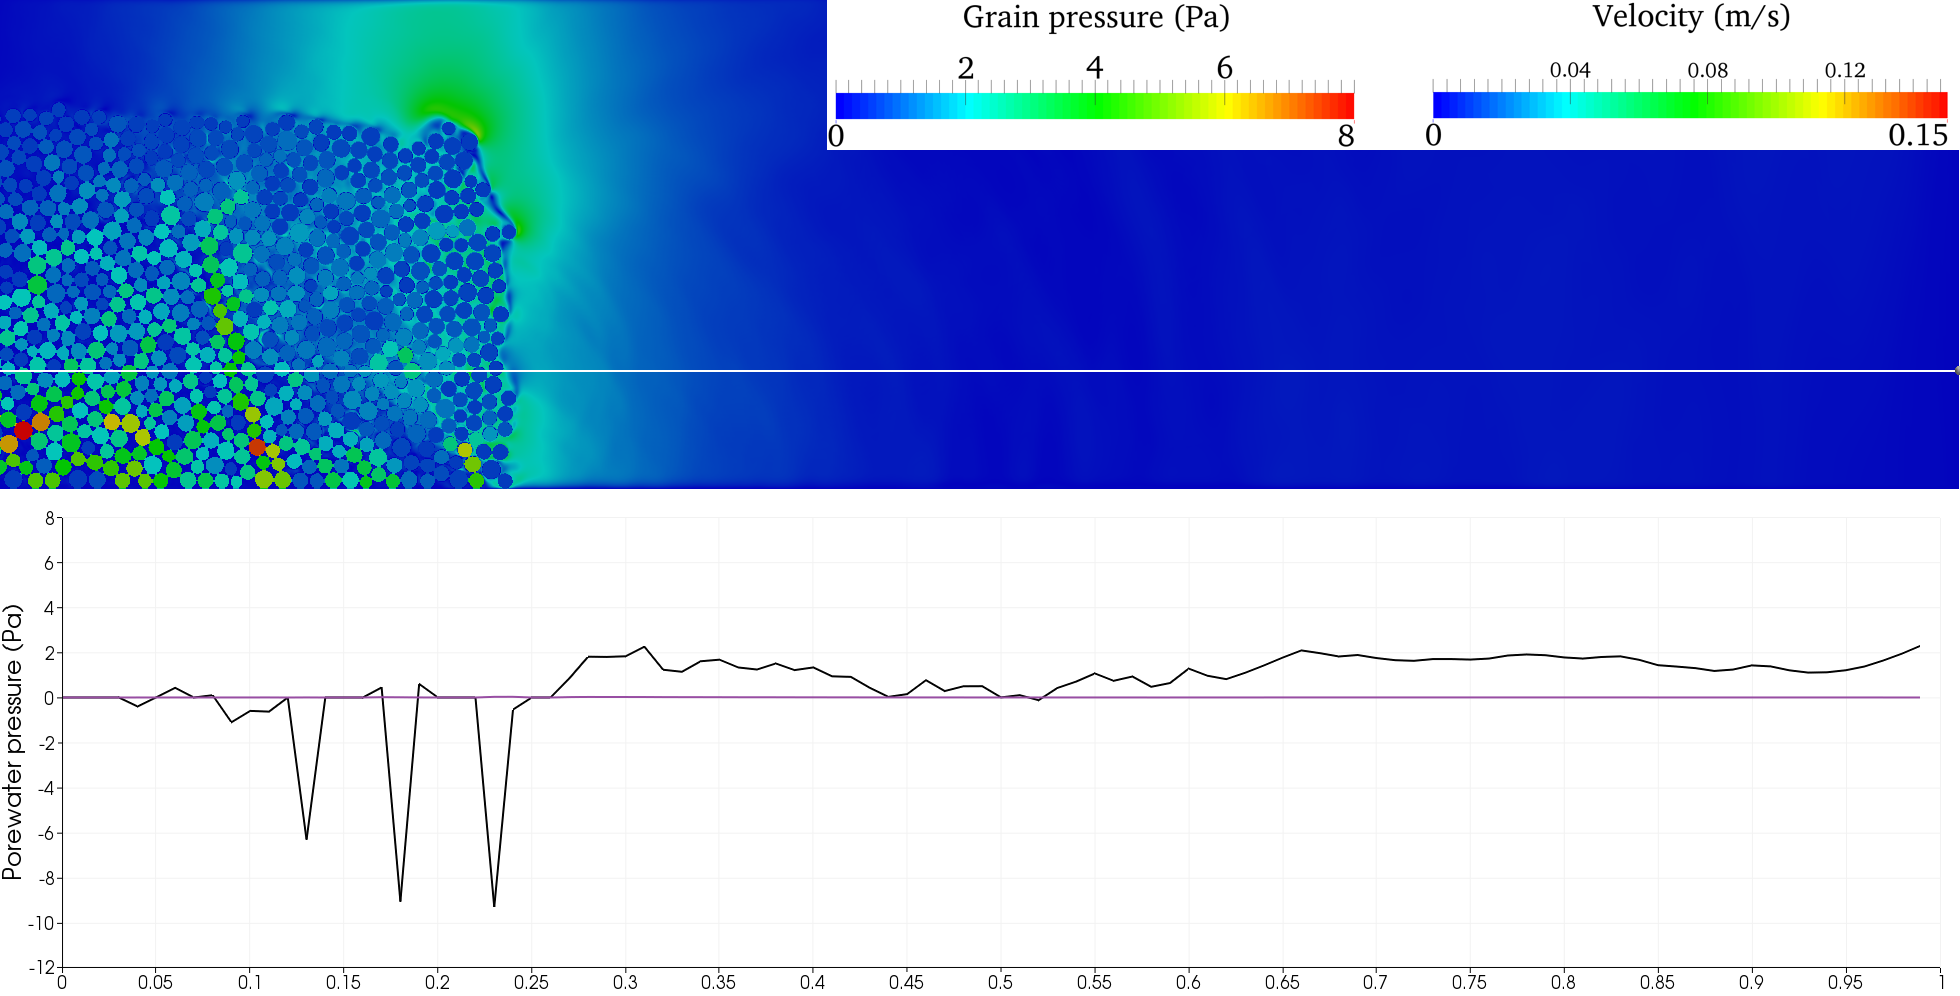
\includegraphics[width=\linewidth]{figs/a08/Loose_r095_PWP_ini}
    \caption{Low permeability (\textit{r} = 0.95 \textit{R}) - Pressure at the 
    bottom of the granular flow.}
    \label{fig:Loose_r095_PWP_ini}
\end{subfigure}
}
\end{figure}
\begin{figure}
\ContinuedFloat
\makebox[\linewidth][c]{
\begin{subfigure}[t]{0.975\linewidth}
	\centering
    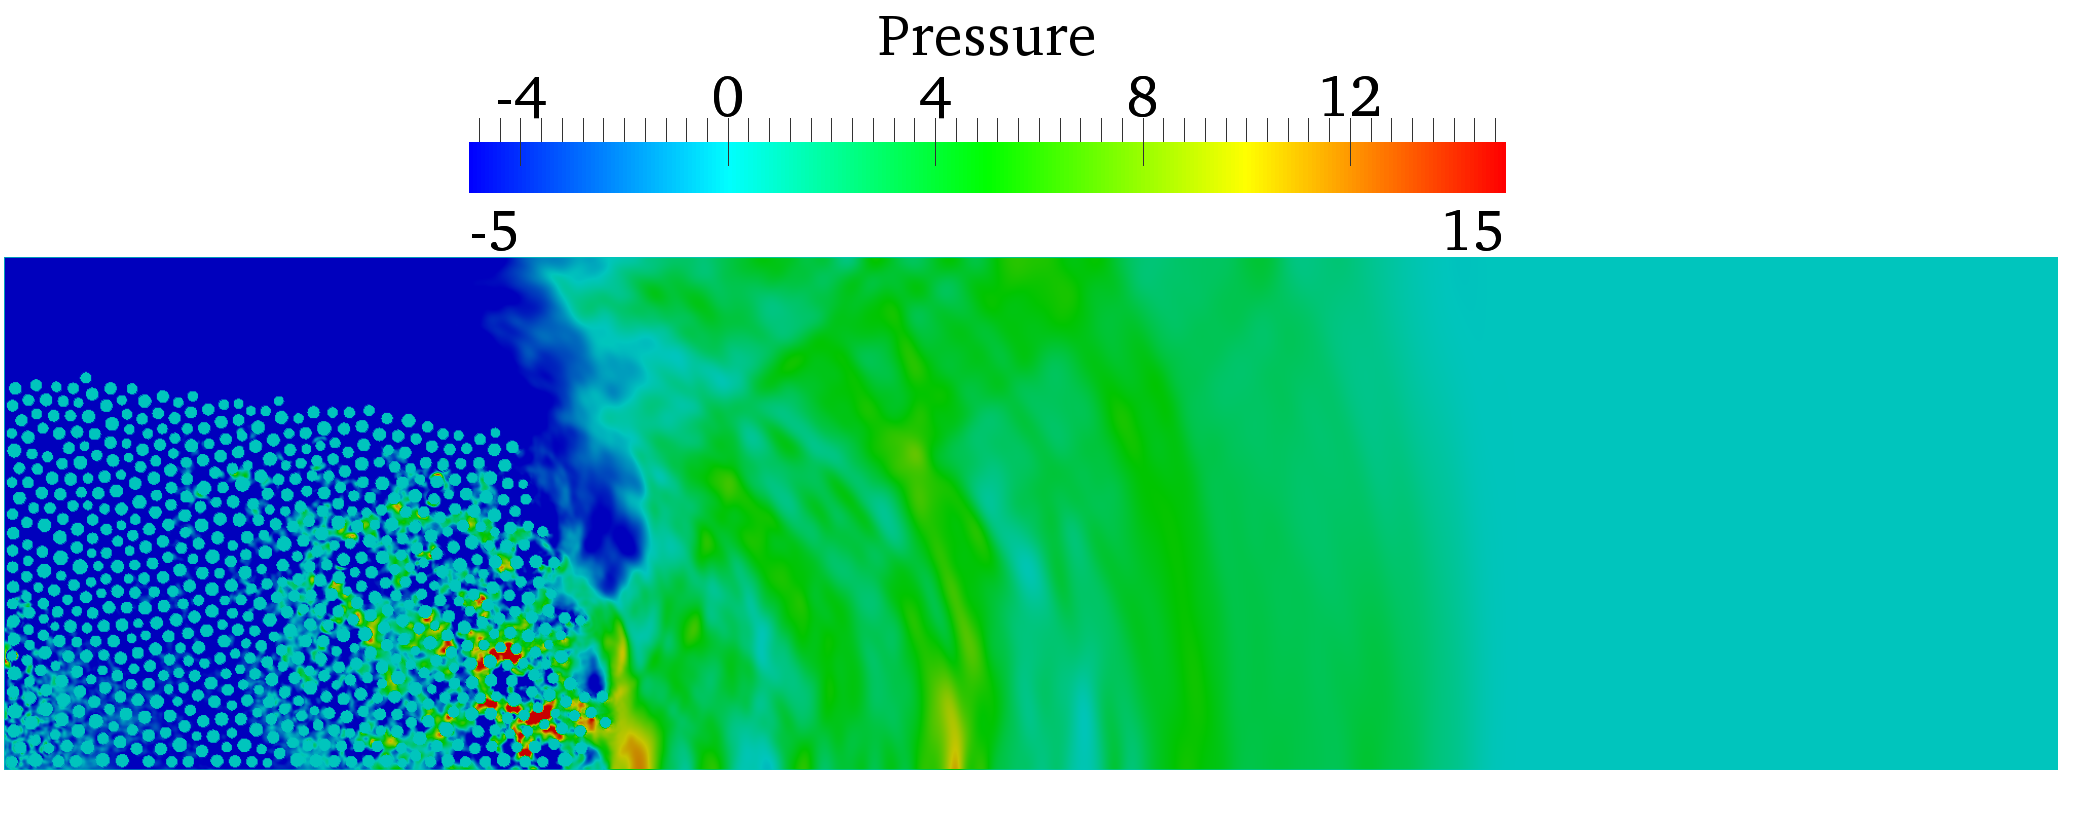
\includegraphics[width=\linewidth]{figs/a08/r07_PWP_ini_press_loose}
    \caption{High permeability (\textit{r} = 0.7 \textit{R}) - Pressure contour 
    (Pa).}
    \label{fig:Loose_r07_PWPress_ini}
\end{subfigure}
}\\
\makebox[\linewidth][c]{
\begin{subfigure}[t]{0.975\linewidth}
	\centering
    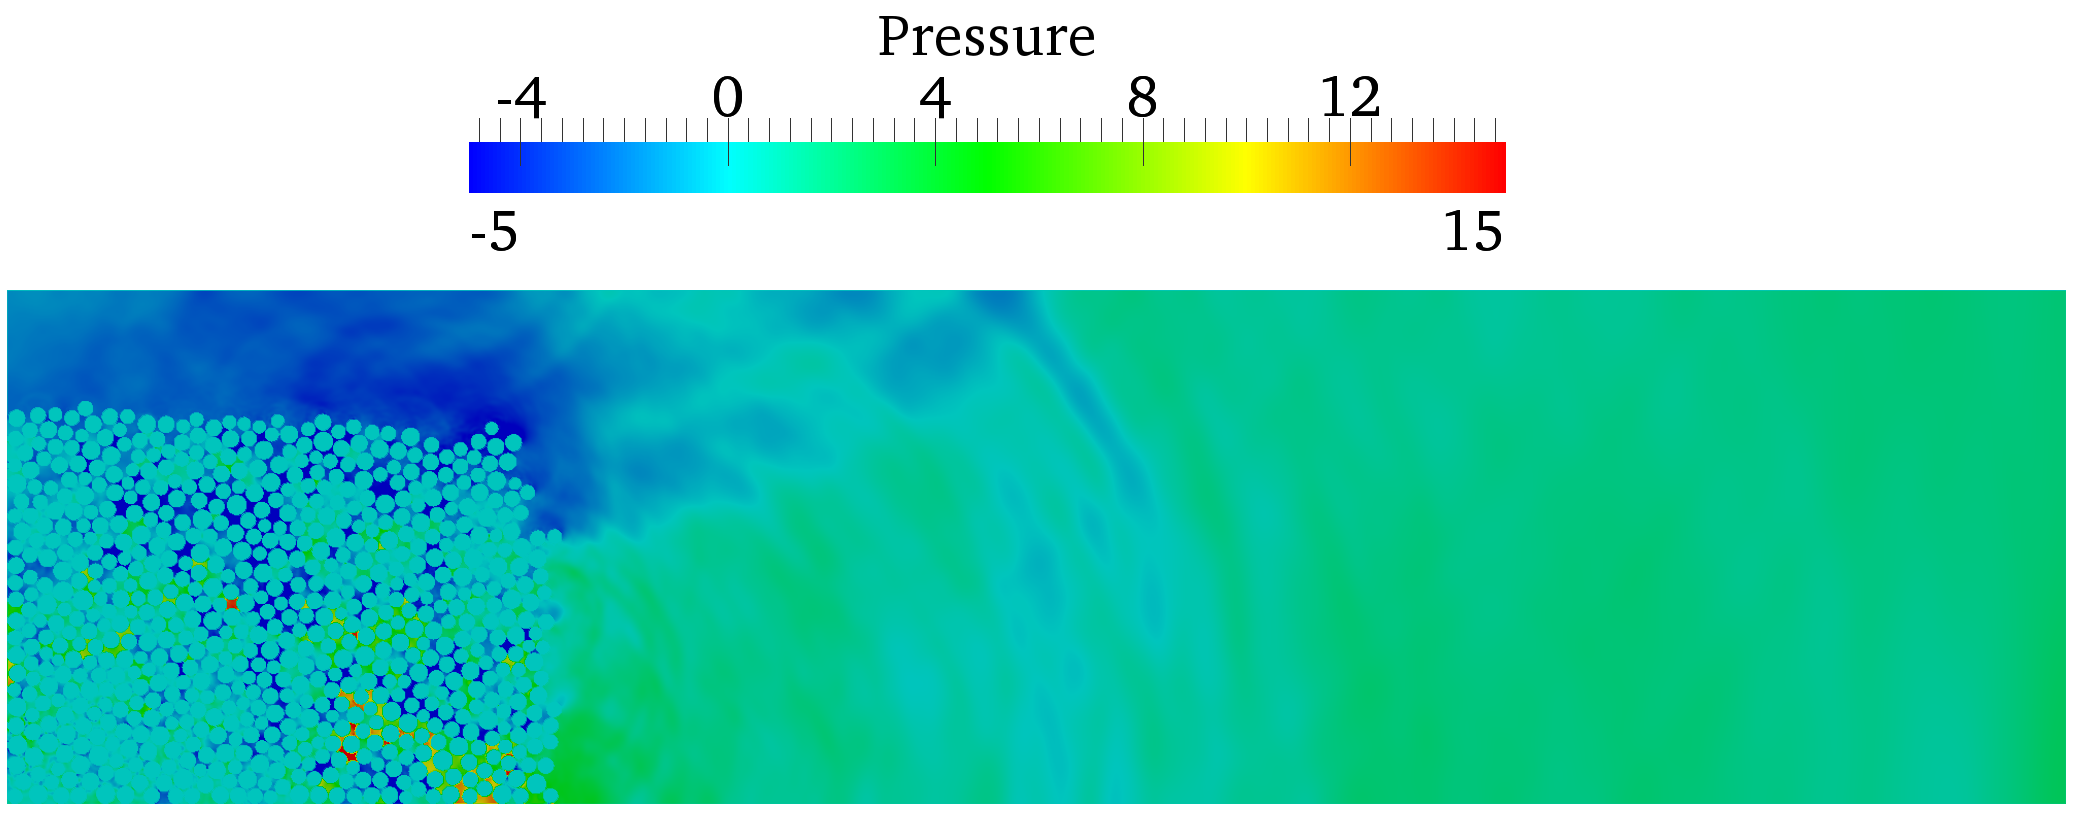
\includegraphics[width=\linewidth]{figs/a08/r095_PWP_ini_press_loose}
    \caption{Low permeability (\textit{r} = 0.95 \textit{R}) - Pressure contour 
    (Pa).}
    \label{fig:Loose_r095_PWPress_ini}
\end{subfigure}
}
\caption{Effect of permeability on the excess pore water pressure distribution 
along the base of a granular column collapse in fluid (a = 0.8 \& loose 
packing) at $t = \tau_c$.}
\label{fig:Loose_PWP_ini}
\end{figure}

\begin{figure}
\centering
\makebox[\linewidth][c]{
\begin{subfigure}[t]{0.975\linewidth}
	\centering
    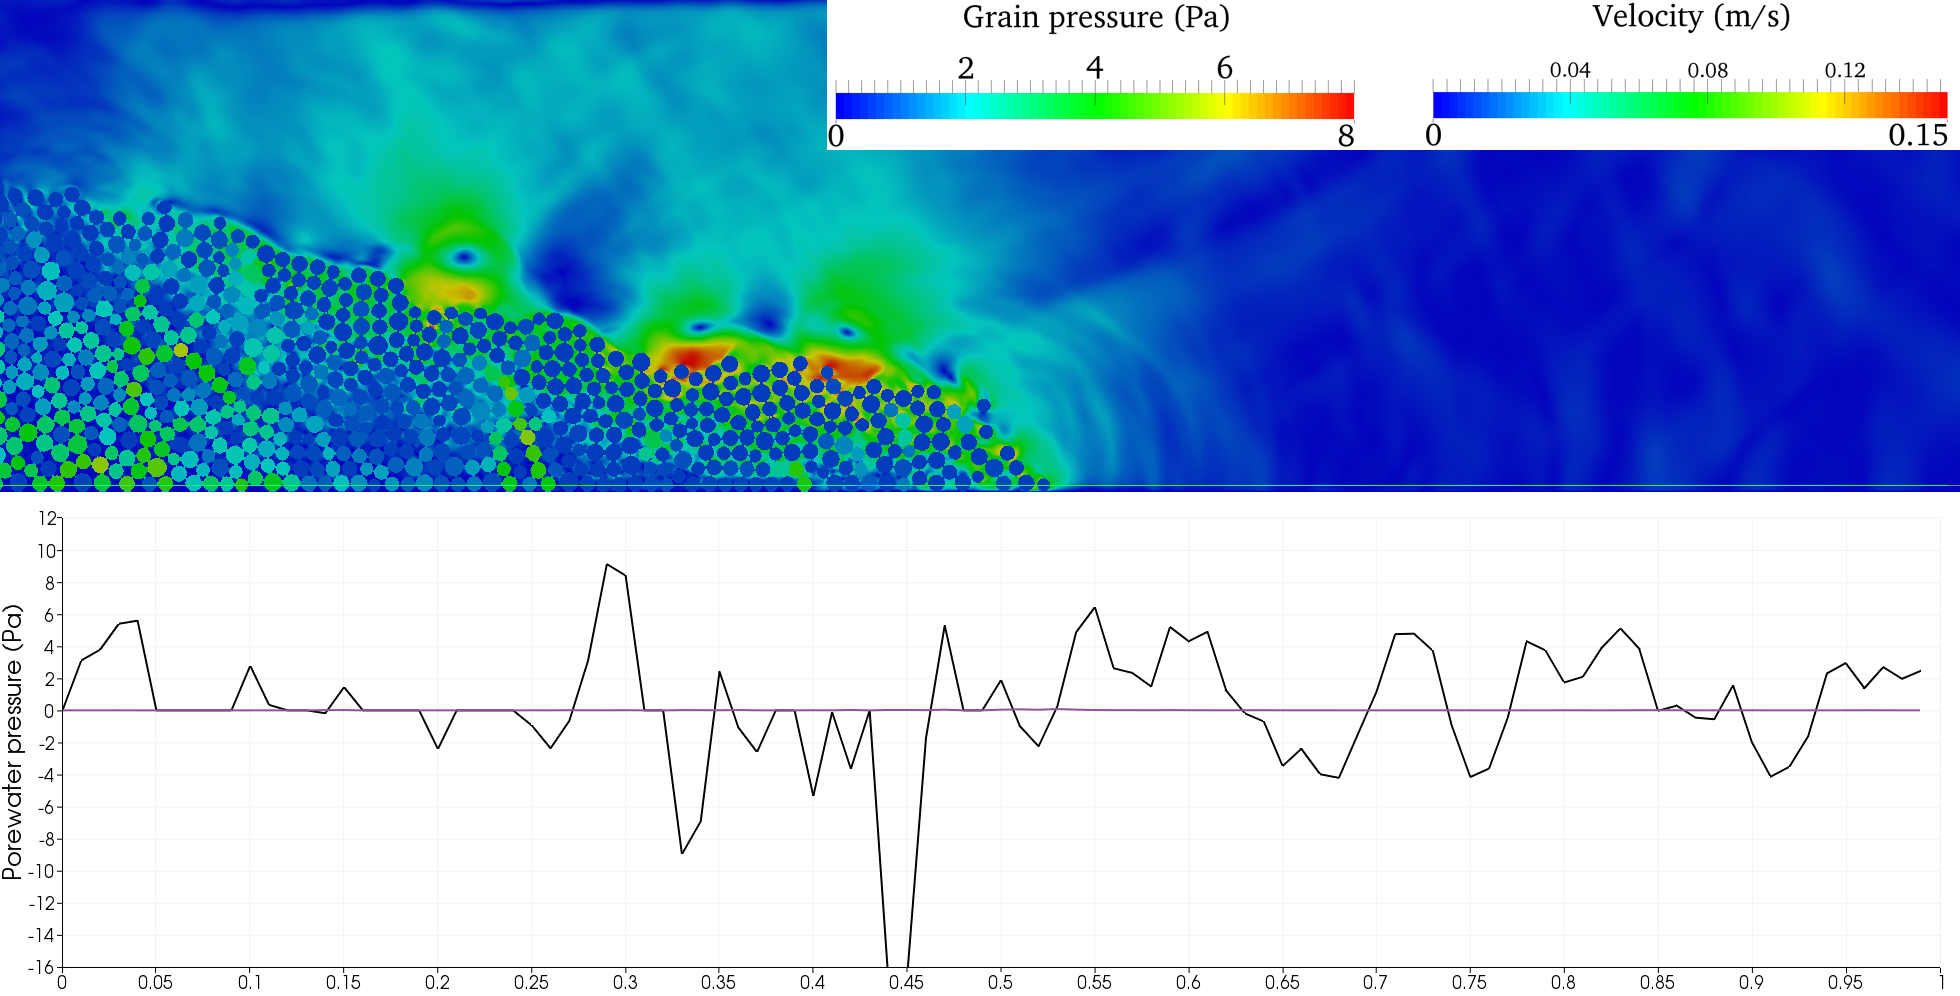
\includegraphics[width=\linewidth]{figs/a08/Loose_r07_PWP_flow}
    \caption{High permeability (\textit{r} = 0.7 \textit{R}) - Pressure at the 
        bottom of the granular flow.}
    \label{fig:Loose_r07_PWP_flow}
\end{subfigure}
}\\
\makebox[\linewidth][c]{
\begin{subfigure}[t]{0.975\linewidth}
	\centering
    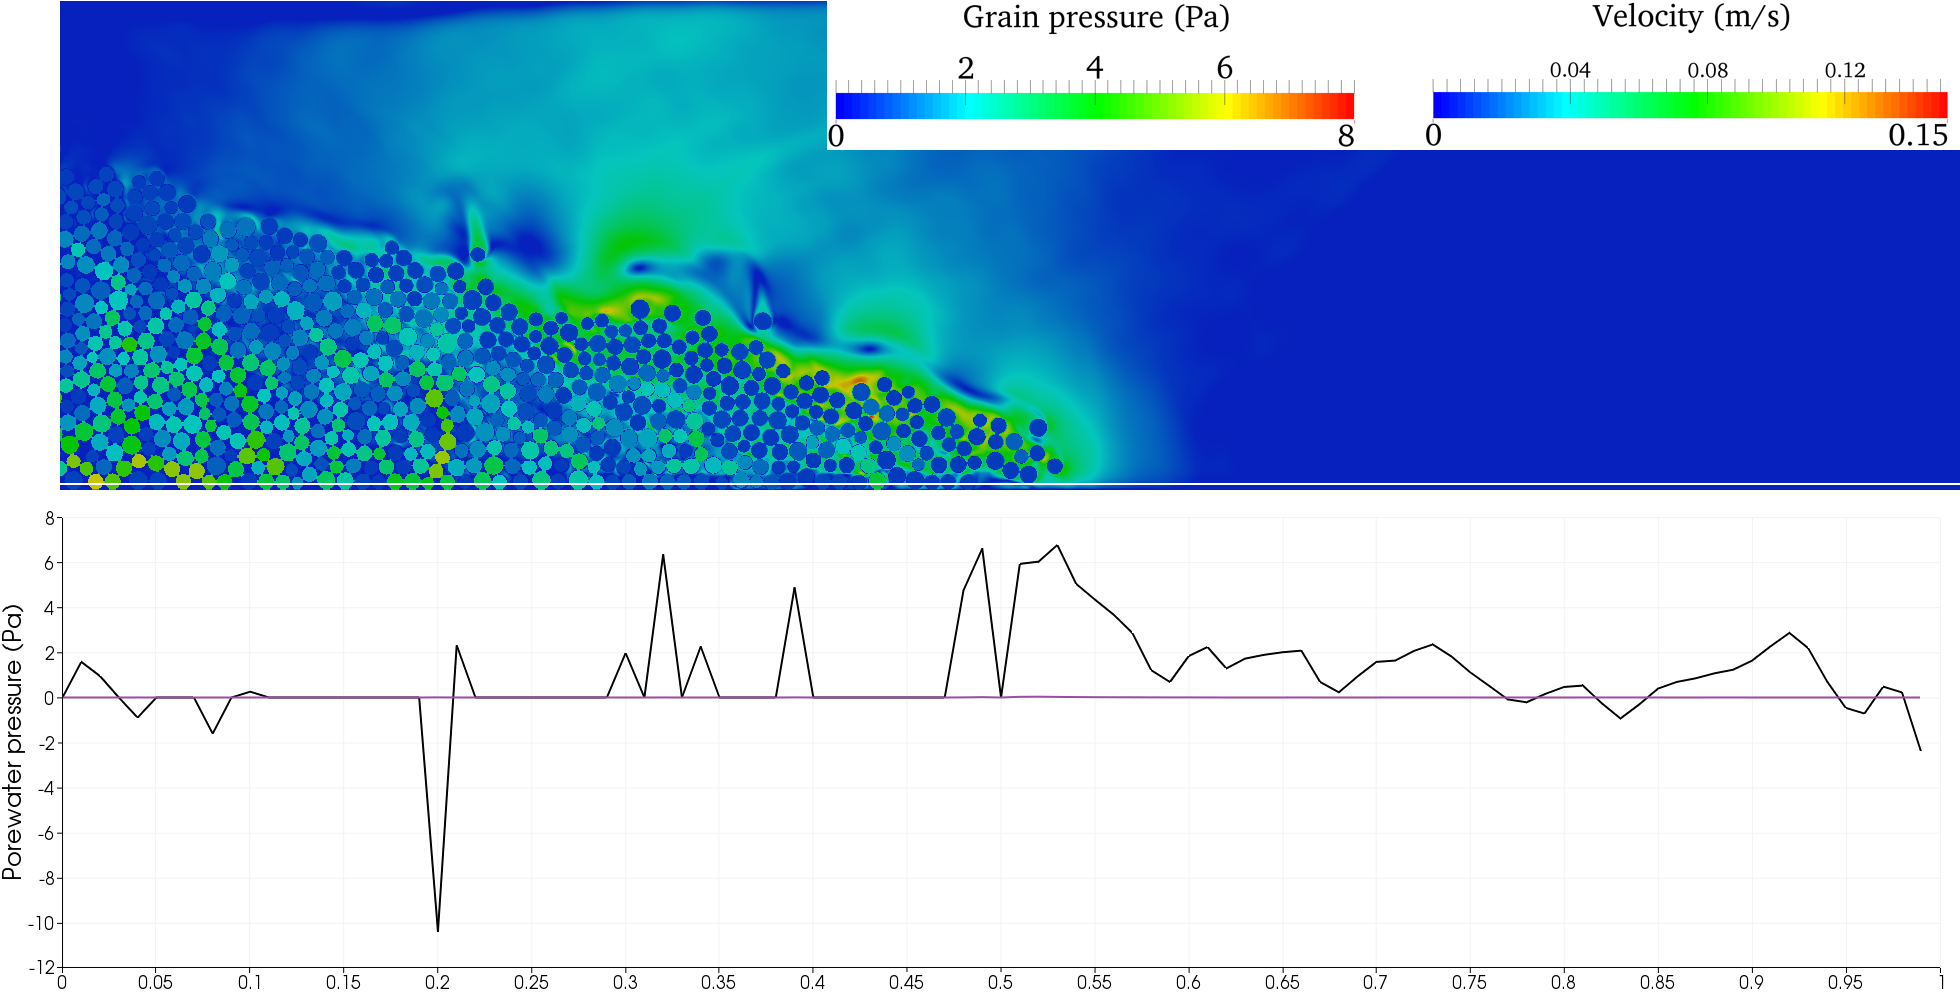
\includegraphics[width=\linewidth]{figs/a08/Loose_r095_PWP_flow}
    \caption{Low permeability (\textit{r} = 0.95 \textit{R}) - Pressure at the 
        bottom of the granular flow.}
    \label{fig:Loose_r095_PWP_flow}
\end{subfigure}
}
\end{figure}
\begin{figure}
\ContinuedFloat
\makebox[\linewidth][c]{
\begin{subfigure}[t]{0.975\linewidth}
	\centering
    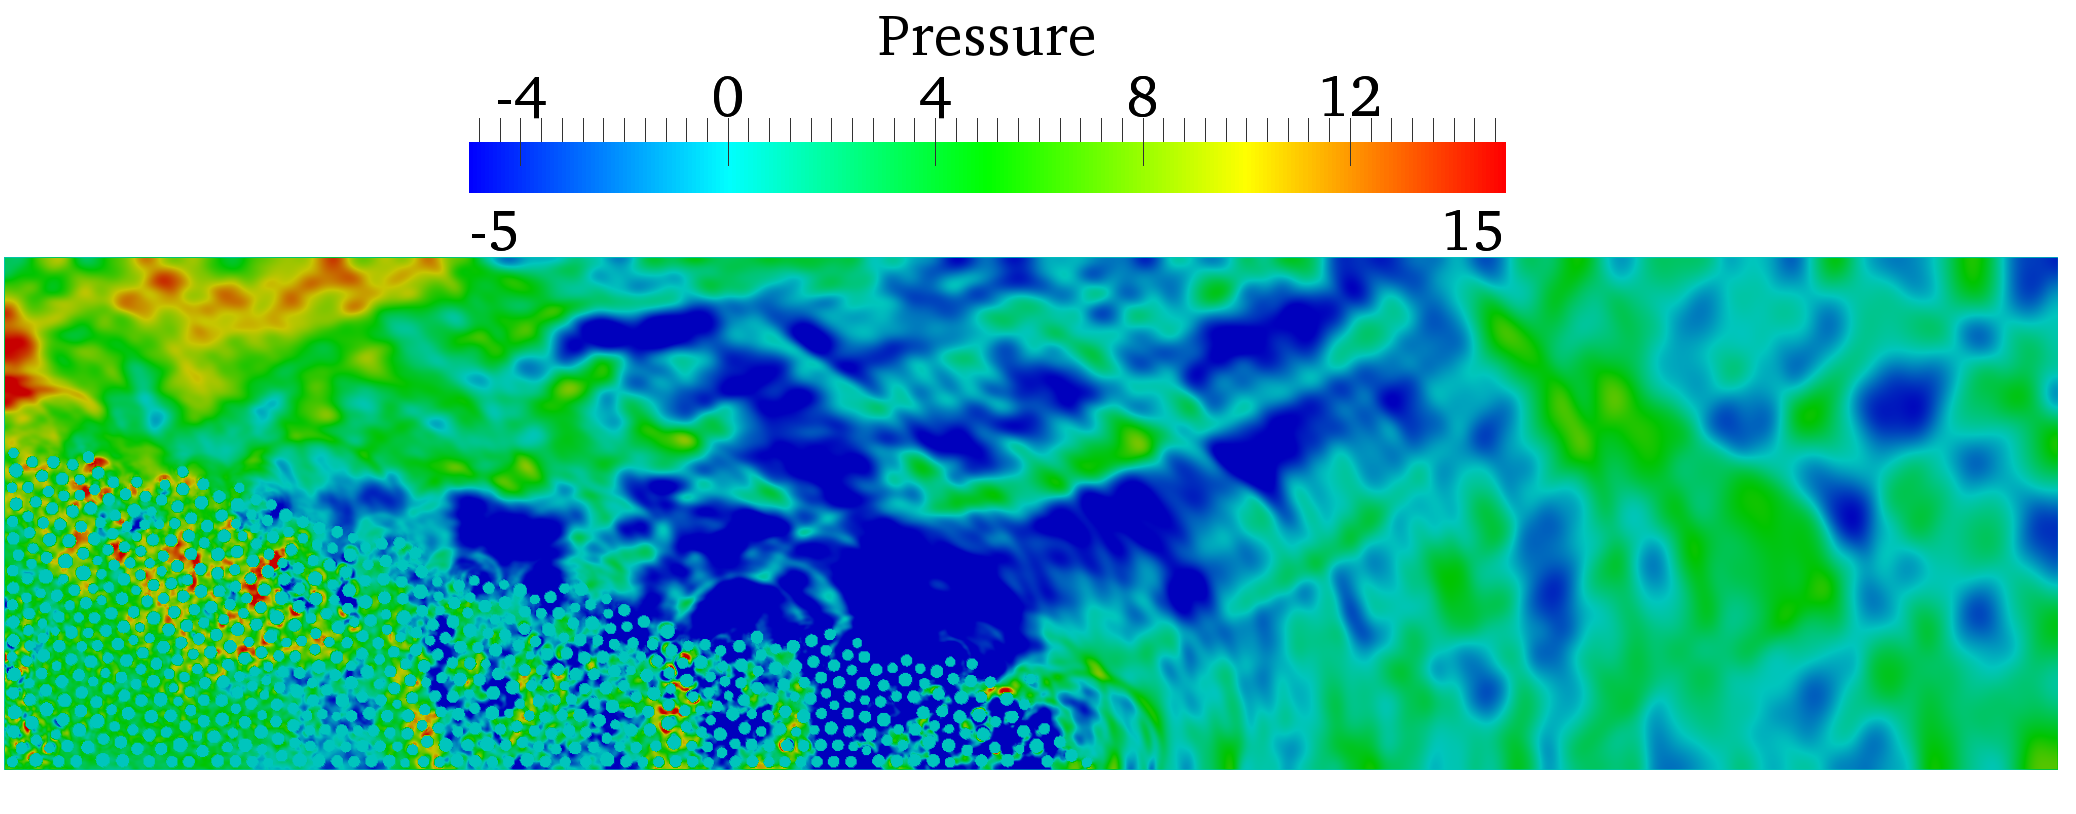
\includegraphics[width=\linewidth]{figs/a08/r07_PWP_flow_press_loose}
    \caption{High permeability (\textit{r} = 0.7 \textit{R}) - Pressure contour 
    (Pa).}
    \label{fig:Loose_r07_PWPress_flow}
\end{subfigure}
}\\
\makebox[\linewidth][c]{
\begin{subfigure}[t]{0.975\linewidth}
	\centering
    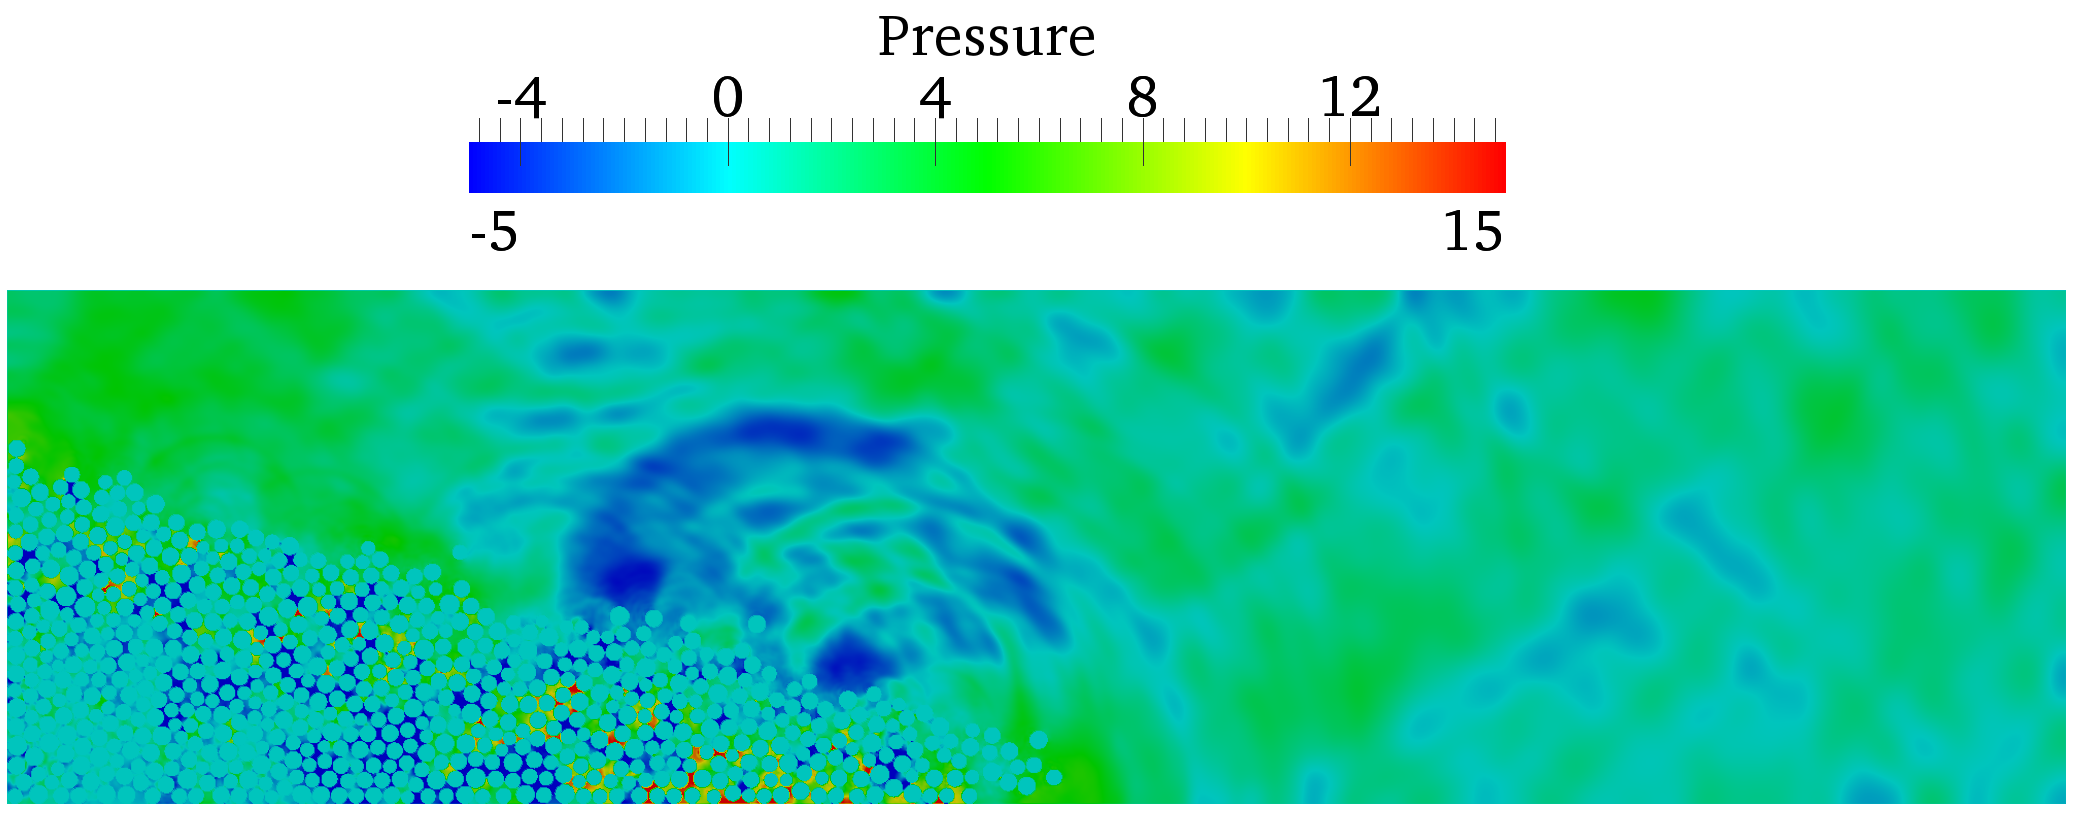
\includegraphics[width=\linewidth]{figs/a08/r095_PWP_flow_press_loose}
    \caption{Low permeability (\textit{r} = 0.95 \textit{R}) - Pressure contour 
    (Pa).}
    \label{fig:Loose_r095_PWPress_flow}
\end{subfigure}
}
\caption{Effect of permeability on the excess pore water pressure distribution 
for a granular column collapse in fluid (a = 0.8 \& loose packing) at $t = 
2\tau_c$.}
\label{fig:Loose_PWP_flow}
\end{figure}

The evolution of the potential energy with time (\cref{fig:PE_a08_loose}) 
reveals that at a very low permeability (\textit{r} = 0.95 \textit{R}), the 
initial potential energy mobilised is smaller than at \textit{r} = 0.9 
\textit{R}. Also with decreasing permeability, the time required to 
dissipate the negative pore-pressure increases. This results in a shorter 
run-out distance in the case of \textit{r} = 0.95 \textit{R} to that of 
\textit{r} = 0.9 \textit{R}. As the quantity of material destabilised is small, 
the flow is thinner and thus has a high Froude's number 
(0.59).~\Cref{fig:KExy_a08_loose} shows that the peak horizontal kinetic 
velocity observed in the case of \textit{r} = 0.9 \textit{R} is higher than 
\textit{r} = 0.95 \textit{R}. A Froude's number of 0.59 for \textit{r} = 0.9 
\textit{R} is observed in contrast to 0.46 for \textit{r} = 0.95 \textit{R}. 
Both values of hydrodynamic radii result in a Froude's number that indicate the 
occurrence of hydroplaning. However, the difference in the amount of material 
destabilised for \textit{r} = 0.95 \textit{R} and the decreased effect of 
hydroplaning results in a shorter run-out distance for \textit{r} = 0.95 
\textit{R} in comparison to \textit{r} = 0.9 \textit{R}.


\Cref{fig:Packing_Density_a08_loose} shows the evolution of packing 
fraction with time for different values of permeability. As the column 
collapses, water is entrained at the flow front. This can 
observed by the decrease in the packing fraction during $t = \tau_c$ and $t = 
3\tau_c$. As the flow progresses, the entrained water is expelled and the soil 
grains consolidate to reach a critical packing density at the end of the flow. 
The permeability (i.e., hydrodynamic radius) plays a crucial role in the rate 
of dissipation of the entrained water. As the permeability decreases, the water 
entrained at the flow front takes longer time to be dissipated resulting in 
lubrication of the flow at low permeabilities.~\Cref{fig:Fr_a08_loose} shows 
that the low permeable columns exhibit higher Froude's numbers, greater than 
0.4, that indicates occurrence of hydroplaning. This lubrication effect results 
in an increase in the run-out distance for columns with low permeabilities.

\begin{figure}
	\centering
    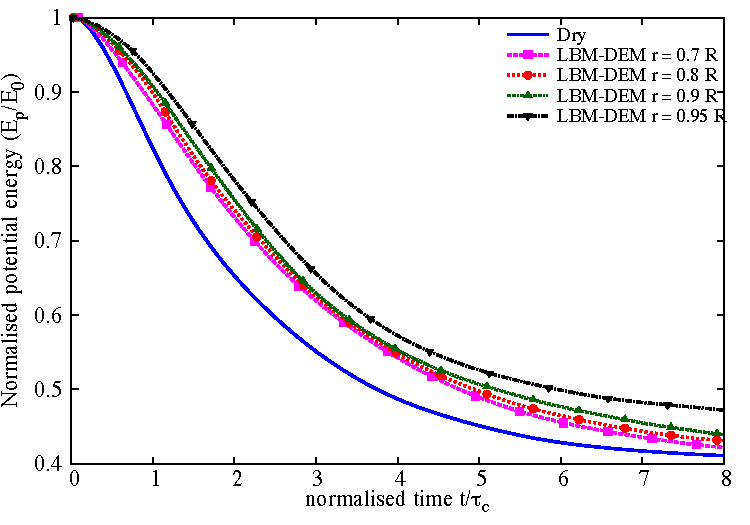
\includegraphics[width=0.8\linewidth]{figs/PE_a08_loose}
    \caption{Effect of permeability on the evolution of the potential energy 
    with time for a granular column collapse in fluid (a = 0.8 \& loose 
    packing).}
    \label{fig:PE_a08_loose}
\end{figure}


\begin{figure}
\centering
\makebox[\linewidth][c]{
\begin{subfigure}[t]{0.8\linewidth}
	\centering
    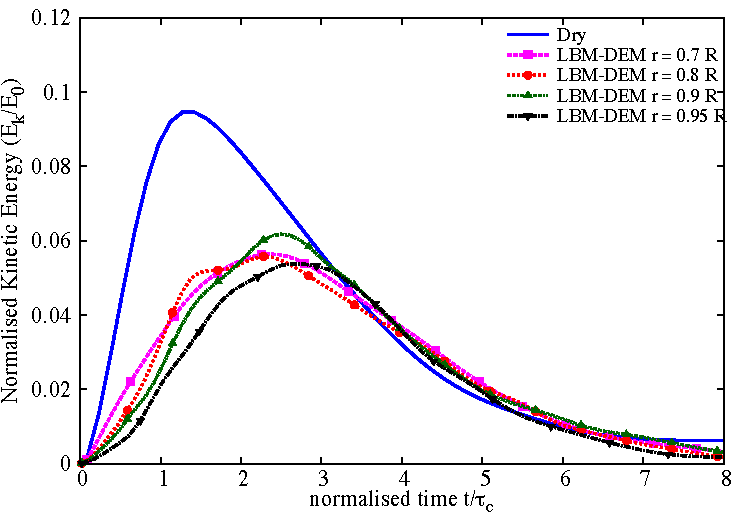
\includegraphics[width=\linewidth]{figs/KE_a08_loose}
    \caption{Evolution of the total kinetic energy.}
    \label{fig:KE_a08_loose}
\end{subfigure}
}\\
\makebox[\linewidth][c]{
\begin{subfigure}[t]{0.95\linewidth}
	\centering
    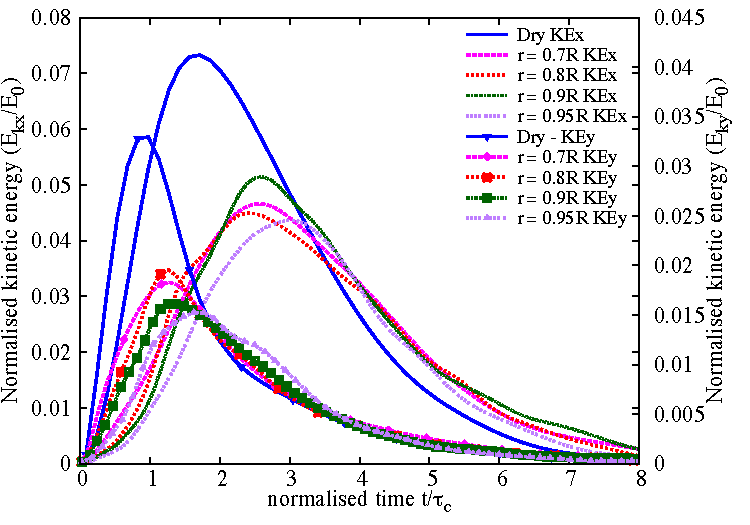
\includegraphics[width=\linewidth]{figs/KExy_a08_loose}
    \caption{Evolution of horizontal and vertical kinetic energies.}
    \label{fig:KExy_a08_loose}
\end{subfigure}
}
\caption{Effect of permeability on the evolution of kinetic energies with time 
for a granular column collapse in fluid (a = 0.8 \& loose packing).}
\label{fig:a08_loose_energy}
\end{figure}

\begin{figure}
\centering
\makebox[\linewidth][c]{
\begin{subfigure}[t]{0.95\linewidth}
	\centering
    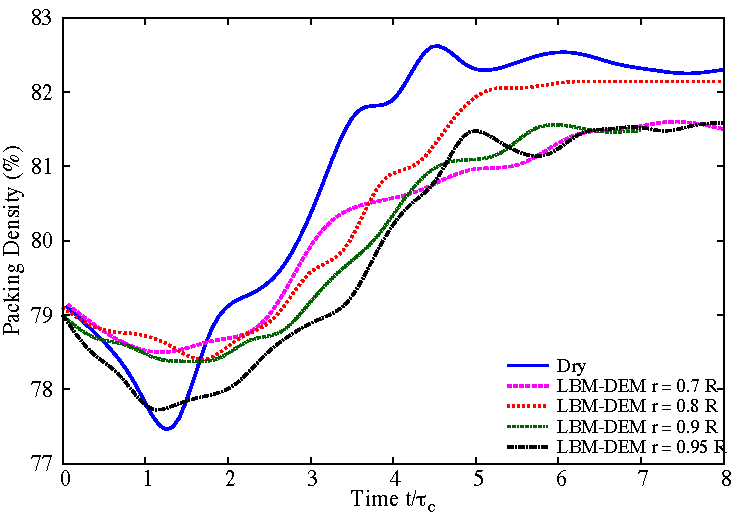
\includegraphics[width=0.8\linewidth]{figs/Packing_Density_a08_loose}
    \caption{Evolution of packing density.}
    \label{fig:Packing_Density_a08_loose}
\end{subfigure}
}\\
\makebox[\linewidth][c]{
\begin{subfigure}[t]{0.95\linewidth}
	\centering
    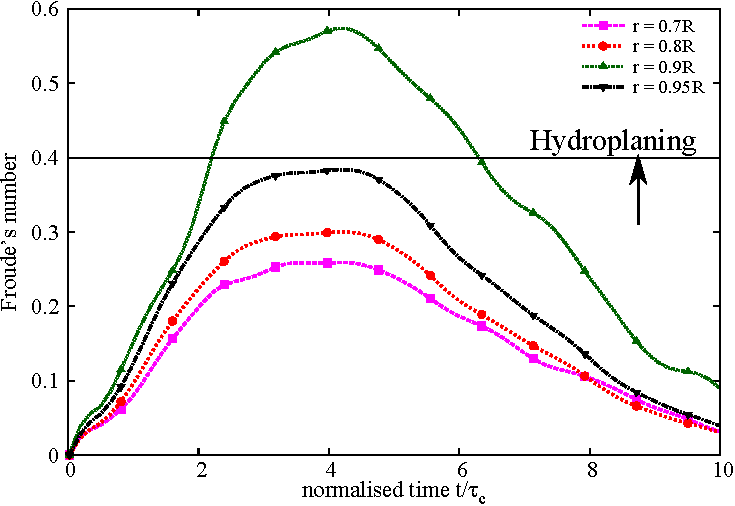
\includegraphics[width=0.8\linewidth]{figs/Fr_a08_loose}
    \caption{Evolution of Froude's number.}
    \label{fig:Fr_a08_loose}
\end{subfigure}
}
    \caption{Effect of permeability on the evolution of packing density and 
    Froude's number for a granular column collapse in fluid (a = 0.8 \& loose 
    initial packing).}
    \label{fig:Packing_Density_Fr_a08_loose}
\end{figure}


The evolution of grain trajectories with time are presented 
in~\cref{fig:Loose_a08_permeability} for low (\textit{r} = 0.95 \textit{R}) and 
high (\textit{r} = 0.9 \textit{R})
permeability conditions. It can be observed that a high 
permeability column shows a parabolic (convex) final profile in contrast to the 
more concave profile observed in low permeability condition, due to the effect 
of drag forces on the flow front. This difference in the flow thickness results 
in a higher value of Froude's number (0.59) and the occurrence of hydroplaning 
in the low permeability condition. Due to the high permeability, the water 
entrained at the flow front is dissipated quicker and 
thus no lubrication effect is observed. A Froude's number of 0.272 (no 
hydroplaning) is observed for the high permeability condition (\textit{r} = 0.7 
\textit{R}). The 
thick flow front in dense condition results in higher effective stress, in 
contrast to the low effective stress in loose condition due to positive 
pore-pressure at the flow front. The higher effective stress results in more 
frictional dissipation in dense condition, while the loose column experiences
lubrication effect. This shows that the drag force predominates at high 
permeability, while the low permeability condition is characterised by 
hydroplaning and lubrication.

\Cref{fig:effective_stress_a08} shows the normalised pressure at the 
base for the low and high permeability flows at $ t = 2\tau_c$. The normalised 
effective stress plotted is obtained as the average over 5 time steps at 
$2\tau_c$. The effective stress at the base is normalised to the effective 
stress of a static granular column before the collapse. A value of 1 indicates 
that the effective stress hasn't changed, which can be observed in the static 
region of the granular column. It can be observed that the normalised effective 
stress is significantly higher for the high permeability condition at the flow 
front in comparison to the almost non-existence of effective stress in the low 
permeability condition. The observation of trivial effective stress at the flow 
front corroborates the lubrication effect observed at low permeability 
conditions.

\begin{figure}
\centering
\makebox[\linewidth][c]{
\begin{subfigure}[t]{0.975\linewidth}
	\centering
    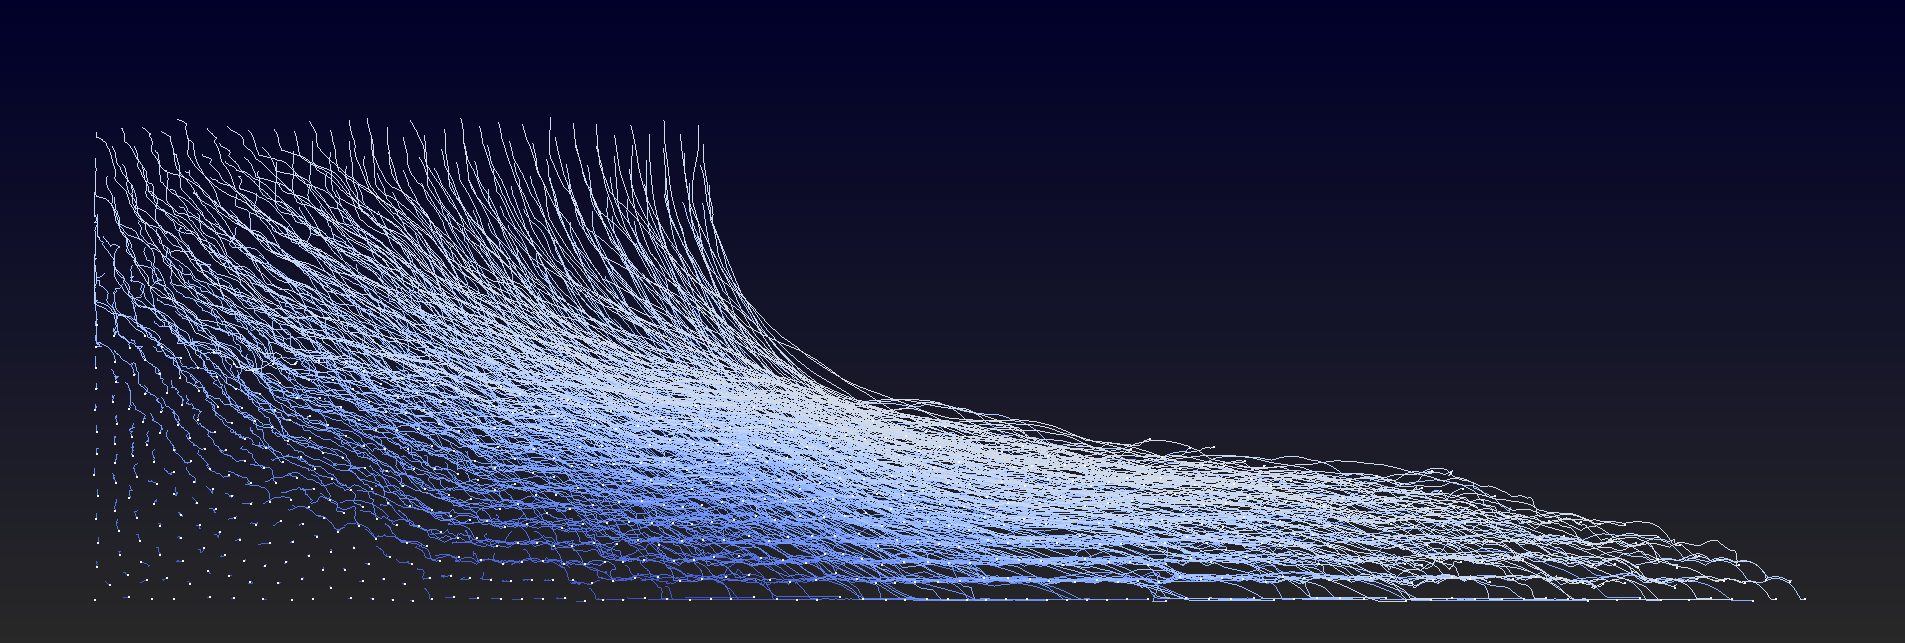
\includegraphics[width=\linewidth]{figs/a08/LBM_MD_loose_a08_r07_pt}
    \caption{High permeability (\textit{r} = 0.7 \textit{R}).}
    \label{fig:LBM_MD_loose_a08_r07_pt}
\end{subfigure}
}\\
\makebox[\linewidth][c]{
\begin{subfigure}[t]{0.975\linewidth}
	\centering
    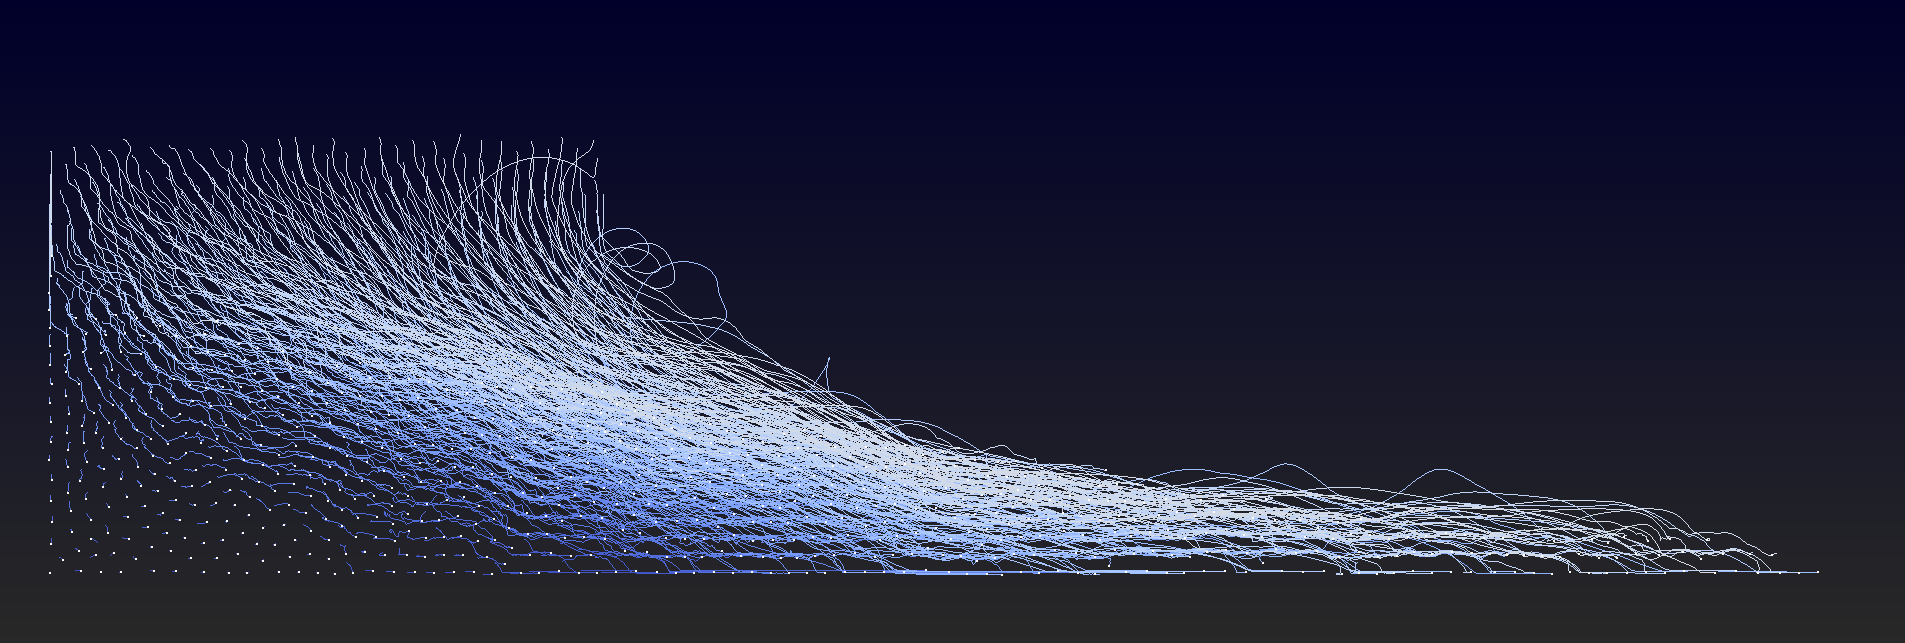
\includegraphics[width=\linewidth]{figs/a08/LBM_MD_a08_Loose_r09}
    \caption{Low permeability (\textit{r} = 0.95 \textit{R}).}
    \label{fig:LBM_MD_a08_Loose_r09}
\end{subfigure}
}
\caption{Particle tracking of the deposit morphology
for a granular column collapse in fluid (a = 0.8 \& loose packing), influence 
of permeability.}
\label{fig:Loose_a08_permeability}
\end{figure}

\begin{figure}
\centering
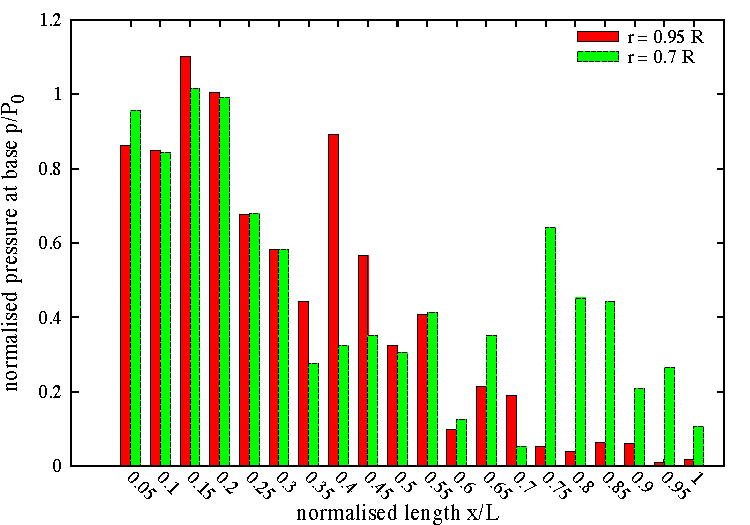
\includegraphics[width=0.97\columnwidth]{figs/a08/effective_stress_a08}
\caption{Effect of permeability on the normalised effective stress for loose 
initial packing at $t = 2\tau_c$.}
\label{fig:effective_stress_a08}
\end{figure}

\Cref{fig:Dense_Loose_PT} shows the grain trajectories of a dense and a loose 
initial packing for a hydrodynamic radius (\textit{r} = 0.95 \textit{R}). It 
can be observed that 
the dense initial packing results in a lot of turbulent behaviour at the flow 
surface in contrast to the more uniform flow behaviour in the loose condition. 
The thickness of the deposit in both dense and loose condition is almost the 
same, however the density of the flow results in a Froude's number of 0.59 and
0.429 for loose and dense conditions, respectively. The low initial density 
results in more hydroplaning in the loose condition. The effect of water 
entrainment at the flow front in dense and loose conditions can be seen 
in~\cref{fig:Dense_Loose_voro}. Water entrainment at the flow front can be 
observed in the loose condition, this is shown by white-coloured (empty Voronoi 
cells) at the flow front. This empty region in the granular packing between the 
granular mass and the base at the flow front represents the entrained water, 
which results in hydroplaning. Comparing the evolution packing densities in 
dense and loose conditions
(\cref{fig:Packing_Density_a08_dense,fig:Packing_Density_a08_loose}) 
reveal almost the same packing density when the flow is fully mobilised. Hence, 
it is the density of the flowing granular mass that controls the influence of 
hydroplaning for a given hydrodynamic radius and initial aspect ratio. A 
loosely packed granular column with low permeability entrains 
more water at the flow front, resulting in a hydroplaning effect that overcomes 
the influence of viscous drag forces and thereby yields a higher run-out 
distance than the dry condition.

\section{Summary}

\citeNP{Rondon2011} also observed that the collapse of a granular column in a 
viscous fluid is mainly controlled by the initial volume fraction and not by 
the aspect ratio of the column. The role of the initial volume fraction 
observed explains the pore pressure feedback mechanism proposed 
by~\citeNP{Schaeffer2008,Iverson2000} in the context of landslides. The 
compaction or dilation of grains can cause additional stress in the grains 
which can stabilise or destabilise the soil. The flow is thus controlled by the 
coupling between the dilatancy of the granular layer and the development of 
pore pressure in the fluid phase~\cite{Pailha2008}. The dense column needs to 
dilate in order to flow. When it starts to fall, liquid is then sucked into the 
column, which is then stabilised by the additional viscous 
drag~\cite{Rondon2011,Topin2012}. By opposition the loose column when 
it starts flowing expands and ejects liquid, leading to a partial fluidisation 
of the material.

\begin{figure}[htbp]
\centering
\makebox[\linewidth][c]{
\begin{subfigure}[t]{0.975\linewidth}
	\centering
    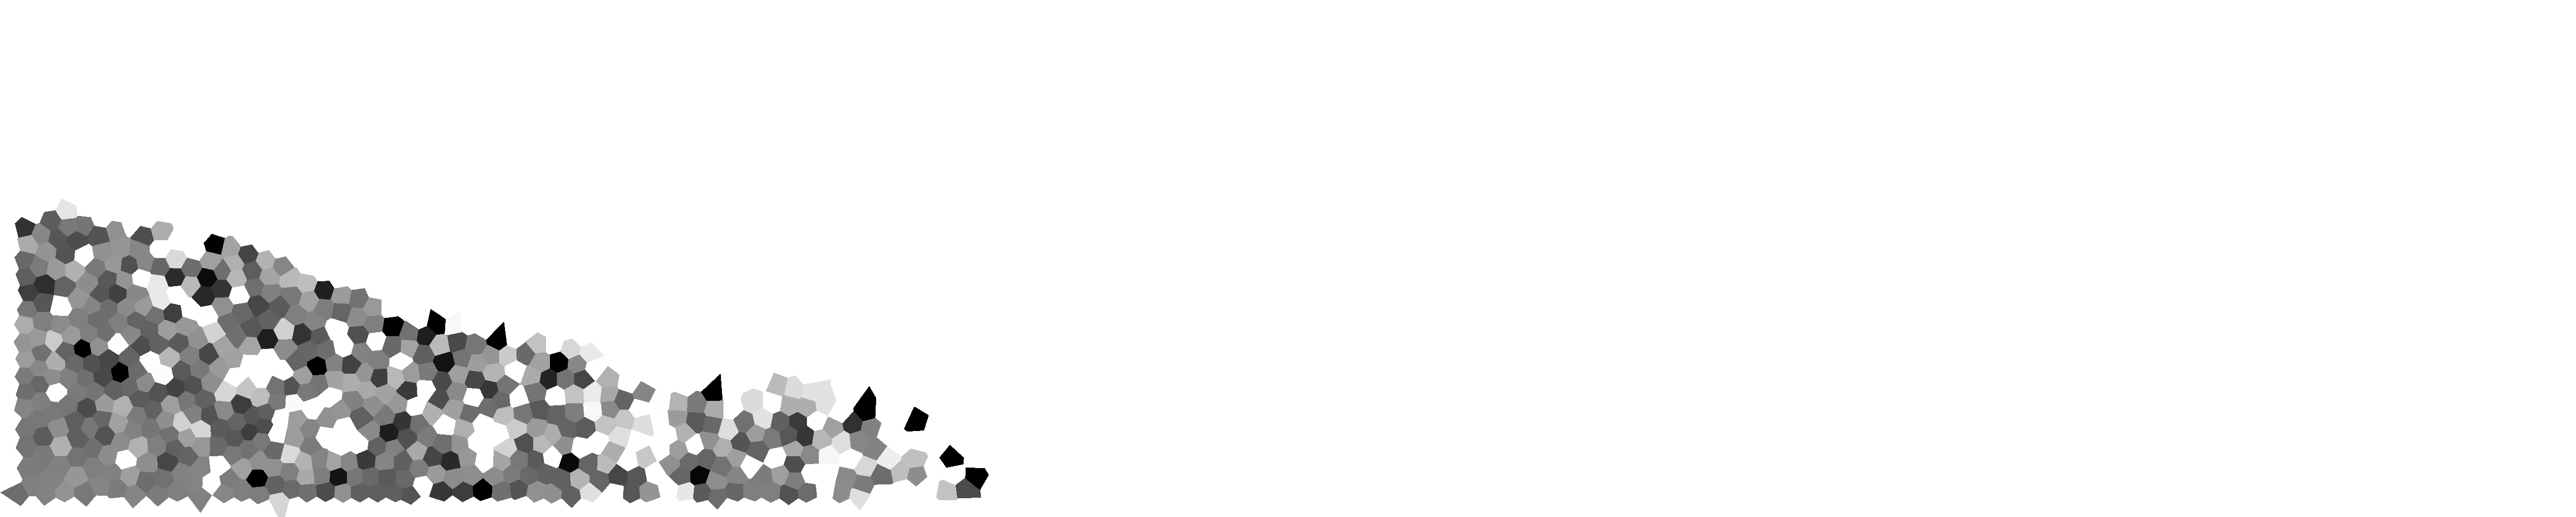
\includegraphics[width=\linewidth]{figs/a08/Dense_a08_voro_tc}
    \caption{Dense initial packing (83\%)}
    \label{fig:Dense_a08_voro_tc}
\end{subfigure}
}\\
\makebox[\linewidth][c]{
\begin{subfigure}[t]{0.975\linewidth}
	\centering
    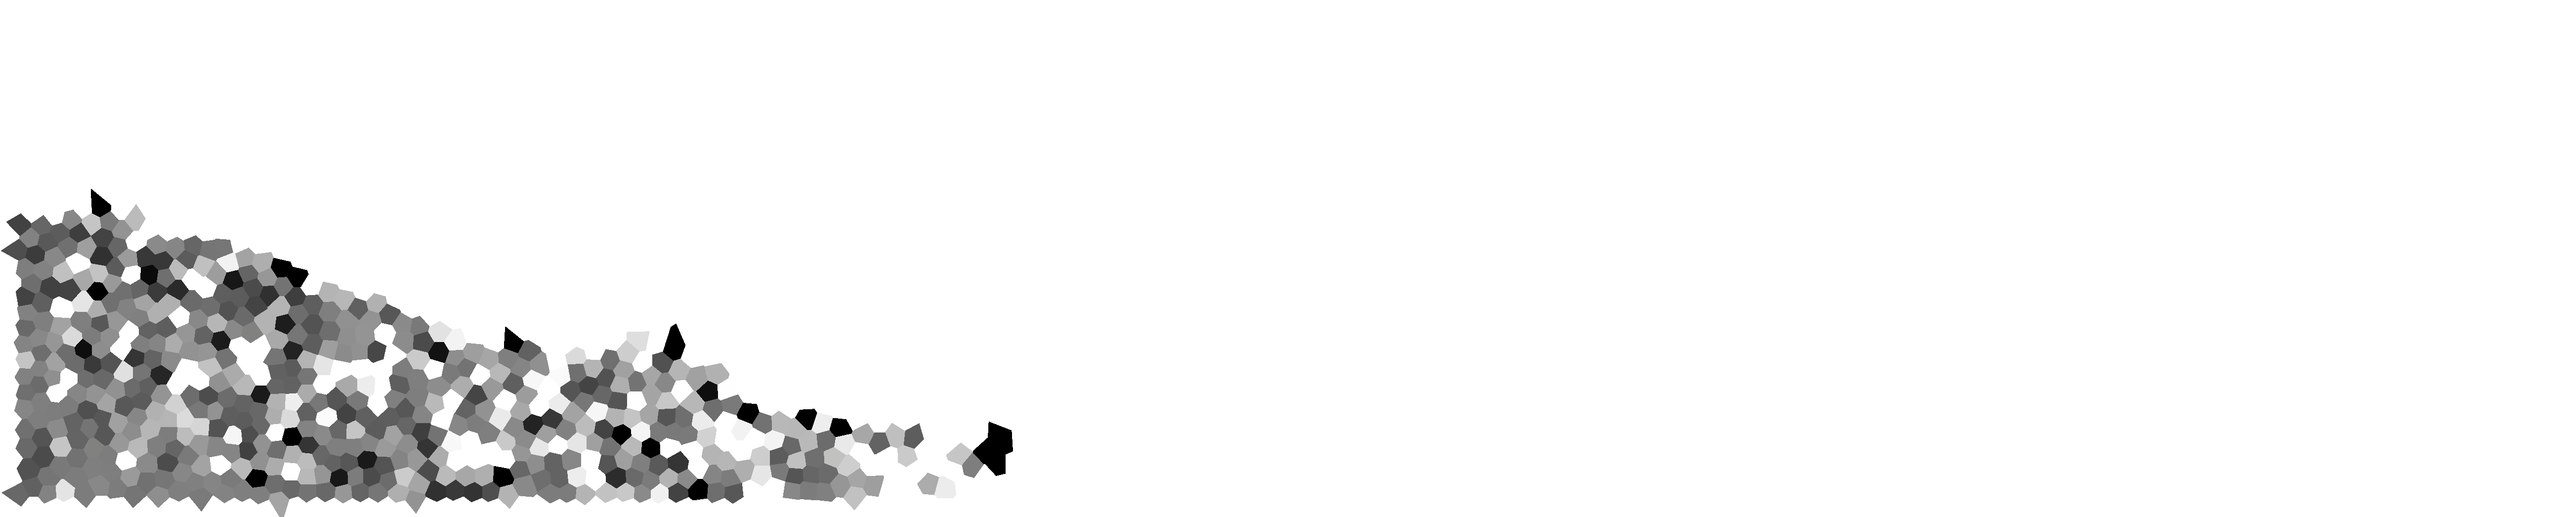
\includegraphics[width=\linewidth]{figs/a08/Loose_a08_voro_tc}
    \caption{Loose initial packing (79\%)}
    \label{fig:Loose_a08_voro_tc}
\end{subfigure}
}
\caption{Evolution of packing fraction at $t = \tau_c$ for dense and loose 
initial packing fraction. Black means dense packing, while white colour denotes 
loose packing in the Voronoi cell.}
\label{fig:Dense_Loose_voro}
\end{figure}

\begin{figure}[htbp]
\centering
\makebox[\linewidth][c]{
\begin{subfigure}[t]{0.8\linewidth}
	\centering
    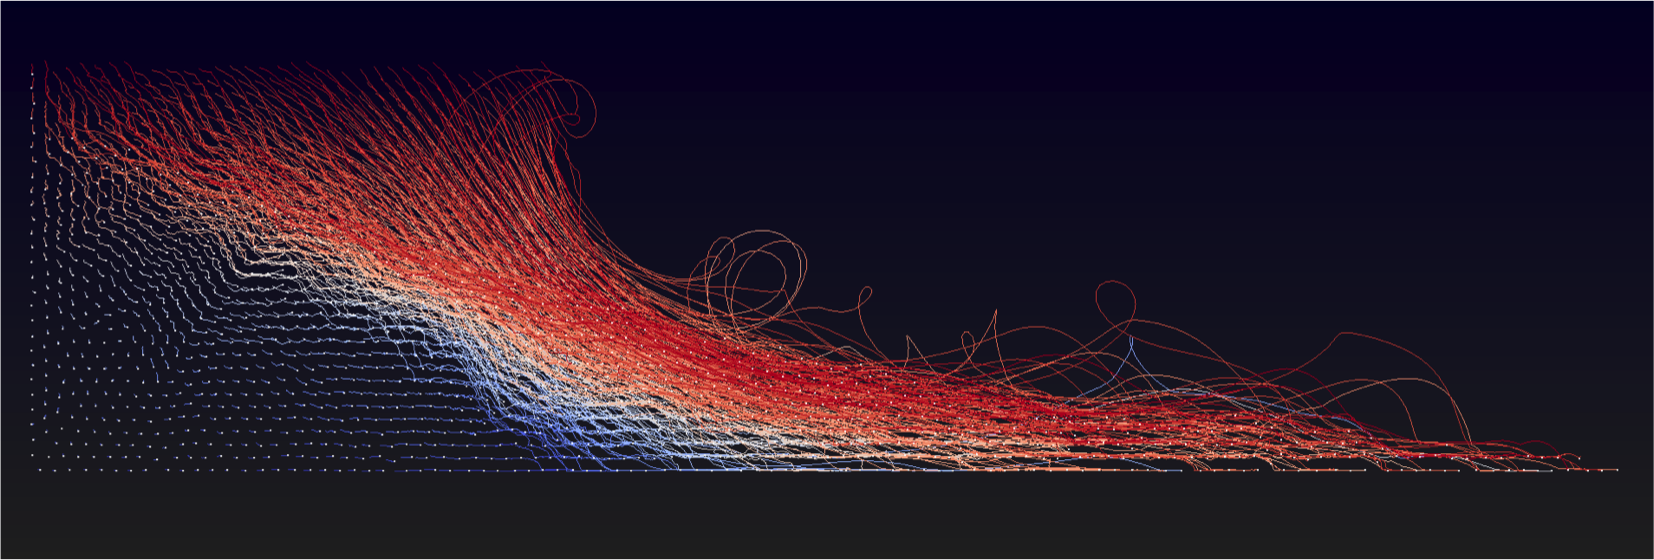
\includegraphics[width=\linewidth]{figs/a08/PT_Dense_R095}
    \caption{Dense initial packing (83\%)}
    \label{fig:PT_Dense_R095}
\end{subfigure}
}\\
\makebox[\linewidth][c]{
\begin{subfigure}[t]{0.8\linewidth}
	\centering
    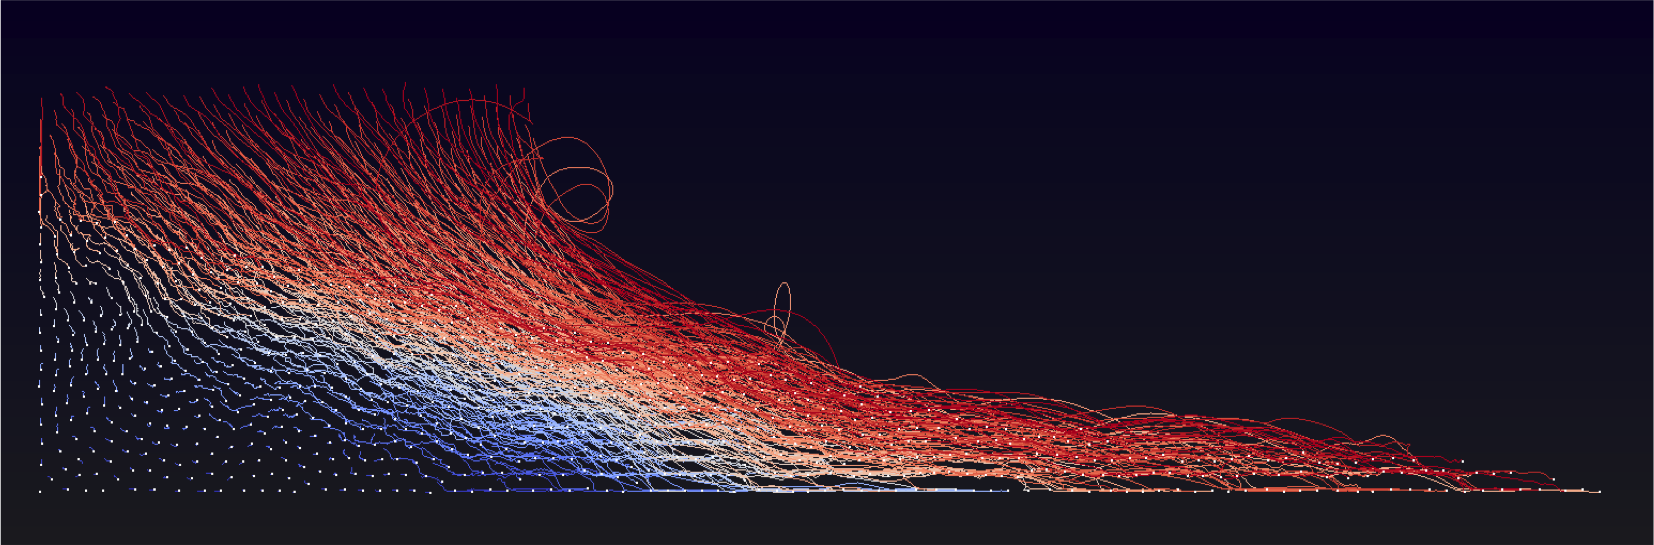
\includegraphics[width=\linewidth]{figs/a08/PT_Loose_R095}
    \caption{Loose initial packing (79\%)}
    \label{fig:PT_Loose_R095}
\end{subfigure}
}
\caption[Effect of initial density on the deposit morphology
for a granular column collapse in fluid (a = 0.8).]{Effect of initial density 
on the deposit morphology
for a granular column collapse in fluid (a = 0.8). Dense vs. loose initial 
packing fraction (\textit{r} = 0.95 \textit{R}). Darker means dense packing, 
white indicates 
loose 
packing density.}
\label{fig:Dense_Loose_PT}
\end{figure}

\bibliographystyle{chicaco}
\bibliography{references}

\end{document}
